%!TEX TS-program = pdflatex
%%*************************************************************************
%% Legal Notice:
%% This code is offered as-is without any warranty either expressed or
%% implied; without even the implied warranty of MERCHANTABILITY or
%% FITNESS FOR A PARTICULAR PURPOSE!
%% User assumes all risk.
%% In no event shall the IEEE or any contributor to this code be liable for
%% any damages or losses, including, but not limited to, incidental,
%% consequential, or any other damages, resulting from the use or misuse
%% of any information contained here.
%%
%% All comments are the opinions of their respective authors and are not
%% necessarily endorsed by the IEEE.
%%
%% This work is distributed under the LaTeX Project Public License (LPPL)
%% ( http://www.latex-project.org/ ) version 1.3, and may be freely used,
%% distributed and modified. A copy of the LPPL, version 1.3, is included
%% in the base LaTeX documentation of all distributions of LaTeX released
%% 2003/12/01 or later.
%% Retain all contribution notices and credits.
%% ** Modified files should be clearly indicated as such, including **
%% ** renaming them and changing author support contact information. **
%%*************************************************************************


\documentclass[10pt,journal]{IEEEtran}

\usepackage[linesnumbered,ruled,vlined]{algorithm2e}
\SetKwInput{KwInput}{Input} % Set the Input
\SetKwInput{KwOutput}{Output} % set the Output

\usepackage{booktabs, multirow}
\usepackage{amsmath}
\usepackage{amssymb}
\usepackage{graphicx}
\usepackage{dblfloatfix}
\usepackage{array}
\usepackage[hidelinks]{hyperref}
\renewcommand\ttdefault{cmtt}

\usepackage[switch]{lineno}

% *** CITATION PACKAGES ***
%
\ifCLASSOPTIONcompsoc
% The IEEE Computer Society needs nocompress option
% requires cite.sty v4.0 or later (November 2003)
\usepackage[nocompress]{cite}
\else
% normal IEEE
\usepackage{cite}
\fi

% *** SUBFIGURE PACKAGES ***

\ifCLASSOPTIONcompsoc
\usepackage[caption=false,font=footnotesize,labelfont=sf,textfont=sf]{subfig}
\else
\usepackage[caption=false,font=footnotesize]{subfig}
\fi
\usepackage{url}

%\raggedbottom

\begin{document}

% \linenumbers % Comment/Uncomment to toggle linenumbers

\title{Evaluation of Transformer Based Neural Network Architecture in Forecasting Pollution Trends}

\author{Pritthijit~Nath, 001810501028, BCSE UG-IV, 2022

%\IEEEcompsocitemizethanks{\IEEEcompsocthanksitem This work was supported by the project entitled - “Participatory and Realtime Pollution Monitoring System For Smart City”, by the Department of Science and Technology, Government of West Bengal, India.}

\IEEEcompsocitemizethanks{\IEEEcompsocthanksitem Pritthijit Nath is affiliated with the Department of Computer Science and Engineering, Jadavpur University, Kolkata, India. (e-mail: pritthijit.nath@ieee.org). This project was performed under the supervision of Prof. Sarbani Roy (email: sarbani.roy@jadavpuruniversity.in).}

%\thanks{Manuscript received April 19, 2005; revised August 26, 2015.}
}


\IEEEtitleabstractindextext{%
\begin{abstract}

With rising pollution concerns in recent times, producing refined and accurate predictions as a part of United Nations Sustainable Development Goals 11 (Sustainable Cities and Communities) and 13 (Climate Action) have gained utmost importance. As new model architectures become available, it becomes difficult for an average policymaker to evaluate various models comprehensively. One such architecture is the Transformer neural network which has shown an exceptional rise in various areas such as natural language processing and computer vision. This paper explores the performance of such a Transformer based neural network ({PolTrans}) in the domain of pollution forecasting. Experiments based on four univariate city pollution datasets (Delhi, Seoul, Skopje and Ulaanbaatar) and two multivariate datasets (Beijing PM${_{2.5}}$ and Beijing PM${_{10}}$) are performed against baselines consisting of widely used statistical, machine learning and deep learning methods. Findings show that although {PolTrans} performs comparatively better compared to existing deep learning methods such as BiDirectional LSTM, LSTM AutoEncoder, etc. for modelling pollution in cities such as Beijing, Delhi and Ulaanbaatar, in the majority of cases, the {PolTrans} architecture lags behind statistical and machine learnings methods such as AutoRegressive Integrated Moving Average ARIMA), Random Forest Regression, Standard Vector Regression (SVR), etc. in the range of 1.5 - 15 units in terms of Root Mean Square Error.


\end{abstract}


\begin{IEEEkeywords}
Deep Learning, Air Quality, Transformer Neural Network, Time-Series
\end{IEEEkeywords}}

\maketitle

\IEEEdisplaynontitleabstractindextext
\IEEEpeerreviewmaketitle


\ifCLASSOPTIONcompsoc
\IEEEraisesectionheading{\section{Introduction}\label{sec:introduction}}
\else
\section{Introduction}
\label{sec:introduction}
\fi

\IEEEPARstart{E}{nvironmental} risk assessment~\cite{Jones.2001} aims to identify the likelihood of future environmental hazards and the long-term effects such events can pose to various communities and urban systems all over the planet. Out of multiple such possible hazards possessing a looming threat to modern human civilization, climate change and air quality degradation have been identified as the ones requiring prominent attention from key stakeholders. With leading nations now declaring urgent action to combat the ongoing climate change a key subject in their future government policies\cite{UN.2015}, the need for leading technological advancements to develop novel solutions to mitigate such climatic risks have become of utmost importance for long-term sustainability related causes. To develop leading edge computational approaches as efforts to address prominent environmental issues, new and exciting research under the umbrella of Computational Sustainability~\cite{Gomes.2019} has gained traction in the last decade. With ideas from Artificial Intelligence (AI) coupled with numerous applications in interdisciplinary domains, research has shown that AI-based computing holds extensive promise in providing key actionable insights that can help society plan new policies to lessen the harm posed by future hazards.

With regards to modelling air quality in urban environments, methods from AI have presently become pervasive in recent times. Various versions of long short term memory (LSTM) networks along with regression models such as standard vector machines (SVM), linear regression coupled with models taken from econometrics such as autoregressive integrated moving average (ARIMA) are widely used in producing estimates with a fair amount of accuracy. Although LSTMs suffer from a lack of data in certain situations~\cite{Nath.2021}, statistical models such as ARIMA and Holt-Winters have been found to perform substantially better in univariate time-series predictions. Advances made originally in the field of Natural Language Processing (NLP) often find key applications especially in time-series modelling. Deep learning based methods such as recurrent neural networks (RNN) and LSTMs often are used in extensive applications such as sentiment analysis, spam detection and document summarization to name a few.

A recent key innovation in seq2seq modelling originally for NLP applications has been the Transformer~\cite{Vaswani.2017} neural network. Unlike LSTMs and RNNs, Transformers eliminate recurrence which helps decrease model complexity and decrease training time as well. Further, due to the presence of independent components, Transformers can be easily parallelized thus improving computation efficiency when dealing with large sequence datasets. Taking motivation of the wide usage in NLP and recent Computer Vision related tasks~\cite{Parmer.2018}, this paper investigates the utility of Transformer neural networks in air quality modelling. Since the original auto-encoder architecture was specially designed for NLP related sequence modelling tasks, this paper builds upon the original model and utilizes a modified version (referred to as {PolTrans} in this paper) which is a modified architecture suited for tasks such as one-step ahead prediction usually used in pollution count estimation. Additionally, this paper also guides a detailed performance comparison of the time-series models used in air quality modelling and explores any relative improvement {PolTrans} provides over widely used baselines.

The organisation of the remaining parts of this paper is as follows : in Section \ref{sec:related-works}, relevant research studies in this field are briefly discussed. Section \ref{sec:model-archi} contains a detailed description of {PolTrans}. The results of the study along with a discussion of the data are laid out in Section \ref{sec:results}. The conclusion and the broad impact of the study are ultimately presented in Section \ref{sec:conclusion}.

\section{Related Works}
\label{sec:related-works}

This section presents a brief survey of related research studies and architectures proposed for temporal modelling of pollution time-series using various learning based methodologies.

\subsubsection{Statistical Learning} Peng et al.~\cite{Peng.2006} thoroughly investigated through a simulation study on air pollution as well as mortality data to compare the efficacies of various statistical approaches with respect to mean squared error. Koo et al.~\cite{Koo.2020} performed a comparative study on air pollution index in Kuala Lumpur using fuzzy time-series models and found them to outperform other approaches in error and computation time. Dominici et al.~\cite{Dominici.2002} used generative-additive models to model time-series concerning air pollution and health effects. They found the estimates to be similar in Poisson regression and strict convergence parameter settings but upward biased in various default convergence counterparts. Reikard ~\cite{Reikard.2019} investigated the prediction performance of various models on SO${_2}$ emissions by the Kilauea volcano in Hawaii and found methods such as ARIMA to produce accurate estimations on daily and hourly granularities. For PM, regressions and simple persistence methods were found to perform better. Fang et al.~\cite{Fang.2016} used Bayesian Model Averaging (BMA) method and reported the GAMM+BMA combination to produce accurate estimates in learning the association between PM${_{10}}$ and mortality.

\subsubsection{Machine Learning} Dincer at al.~\cite{Dincer.2018} reported showing successful forecasting results using a proposed fuzzy based time-series model built on top of Fuzzy K-Medoid clustering algorithm. Shahriar et al.\cite{Shahriar.2020} performed a comparative study of ML methods such as L-SVM, M-SVM Gaussian Process (GP) and Random Forest regression models and reported GP to perform significantly better in predictions of PM${_{2.5}}$ and PM${_{10}}$. Chen et al.~\cite{Chen.2018} found SVMs to produce better results in prediction of CO${_2}$ and TVOCs and were able to outperform GP, M5P and ANNs. Wang et al.~\cite{Wang.2008} et al. developed an improved version of SVM capable of online learning and used the model to estimate pollution levels based on the air pollutant database in Hong Kong. Staffogia et al.~\cite{Staffogia.2019} used an ensemble methodology to establish relationships between PM and satellite land use and meteorological parameters. Their study produces estimates in 1sq. km spatial resolution and reported finding improvements in the addition of small-scale predictors at monitor locations.

\subsubsection{Deep Learning} Espinosa et al.~\cite{Espinosa.2021} based on exactness and robustness criteria compared multiple forecasting models such as 1DCNN, GRU, LSTM along with different linear regression models to create a multi-criteria methodology for air quality prediction. Niska et al.~\cite{Niska.2004} presented the use of parallel genetic algorithm (GA) to design the architecture of MLPs for forecasting NO${_2}$ emissions reported in Helsinki. The findings showed promising results and found GA to be a capable tool in neural network design. Dunea~\cite{Dunea.2015} proposed a wavelet-feed forward neural network architecture to predict pollutants such as O${_3}$, NO${_2}$ and PM. Their study reported improvements in ANN performance with wavelet integration and were found to present positive results for O${_3}$ and NO${_2}$. Soh et.al~\cite{Soh.2018} created an adaptive deep learning model which combined ANNs, CNNs and LSTMs which was used to extract spatio-temporal air quality relations for improved performance. Lei et al.~\cite{Lei.2020} performed a case study using a hybrid approach involving CNNs and Bi-LSTMs for spatio-temporal modelling of pollution counts in Fushung, Liaoning Province in China.

While extensive studies have been organized in the past, the majority of them have focussed on the utility of classical methodologies such as econometric models, shallow ML models and diverse versions of LSTM in emission modelling and forecasting. Due to the inherent nature of pollutant behaviour, majority studies were regional and lacked a global perspective. This paper aims to investigate the utility of a transformer based model {PolTrans} in air quality modelling and how the prediction performance varies with respect to widely used baselines in major pollution risk areas around the world.

\section{Model Architecture}
\label{sec:model-archi}

This section presents a description of the {PolTrans} model architecture outline in Fig. \ref{fig:model-archi}.

\subsection{Input Data Pre-processing}
\subsubsection{In2Out Sequence Modelling}
To convert the time-series data ${P_{data}}$ into a series of sequences for supervised training, a new dataset is engineered from the original data by breaking into chunks using a rolling window ${\lambda_n}$ of size ${n}$. As the window ${\lambda_n}$ is slid over the 1-dimensional time-series ${P_{data}}$, the series $\{{P_{data, k}}\}^{k=n-i-1}_{k=i}$ is taken as the feature vector while ${P_{data, n-i}}$ is made to serve as the label for the ${i}$~th row of the new dataset. Here, ${1 \leq i \leq {T - n + 1}}$ where ${T}$ stands for the number of time-steps present in ${P_{data}}$. The new dataset ${Q_{data}}$ can be then split and sampled into training, validation and test sets for evaluation purposes as and when needed.

\begin{figure}[h]
\centering
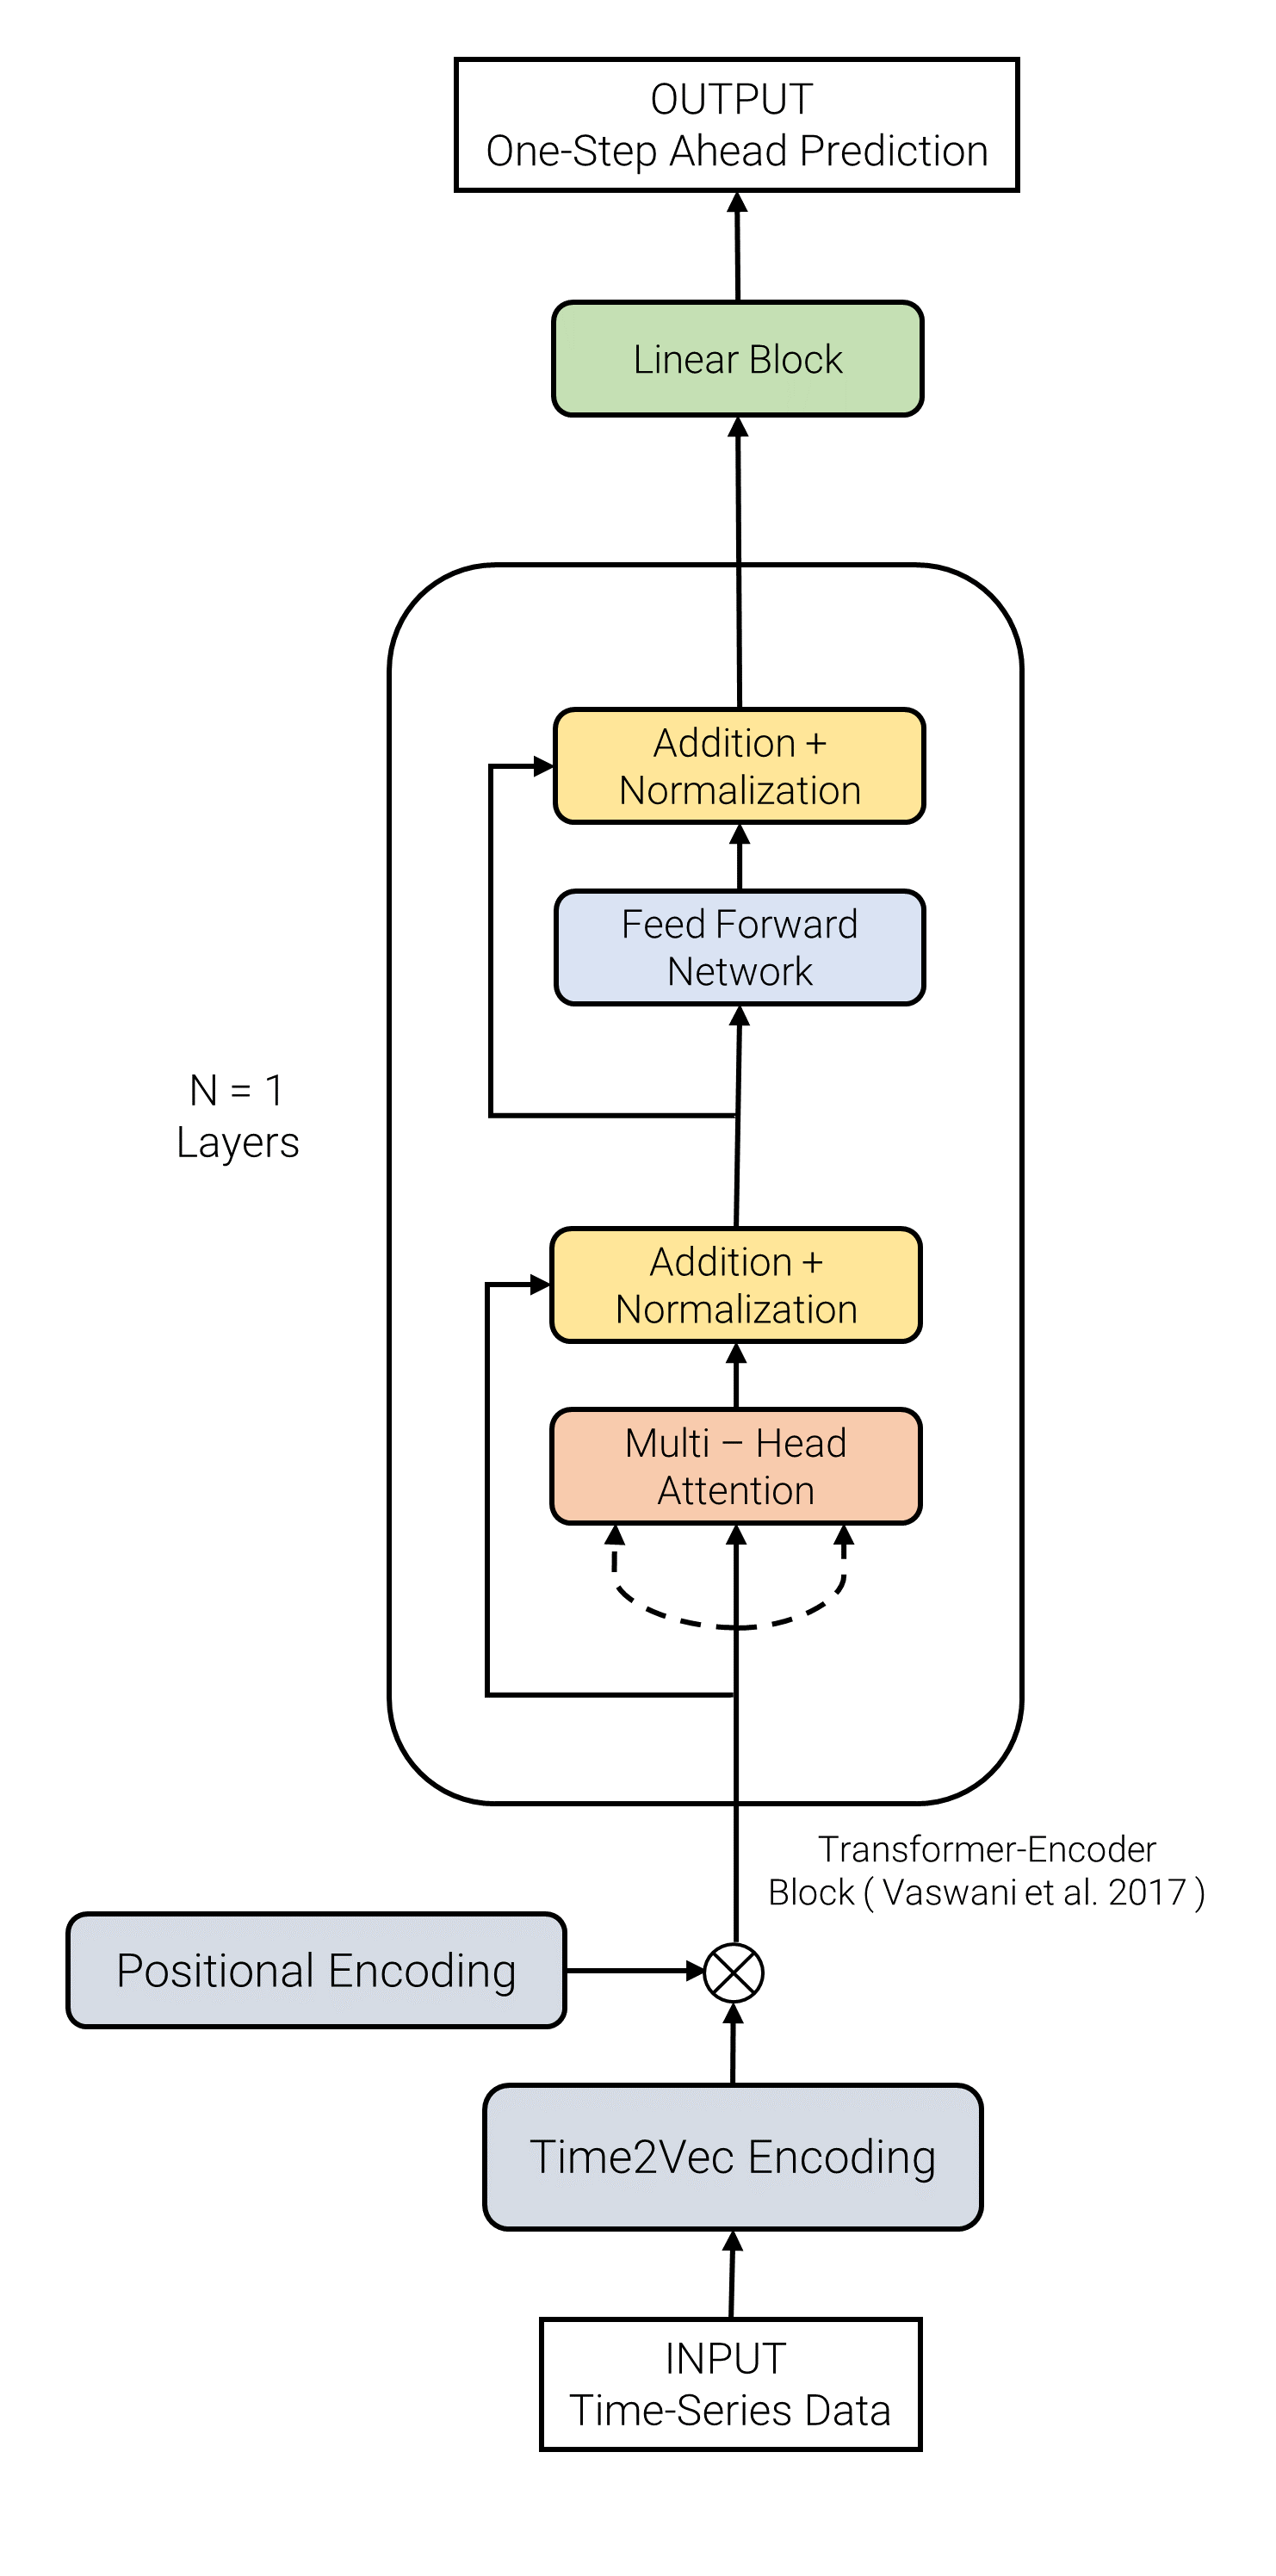
\includegraphics[height=12cm]{../paper_figures/model-architecture.png}
\caption{{PolTrans} model architecture describing the flow of input, application of two kinds of encoding, modelling through the Transformer-Encoder block and output result as a one-step ahead forecast from the last linear block}
\label{fig:model-archi}
\end{figure}

\subsubsection{Time2Vec Encoding}
To create a model agnostic vector representation of time, the supervised feature vectors are passed through the Time2Vec~\cite{Kazemi.2019} Encoding layer. For a scalar time notion ${\tau}$, the resulting Time2Vec encoding ${\mathbf{t} 2 \mathbf{v}(\tau)}$ is a vector of size ${n}$ that can be defined as follows:

\begin{equation}
\mathbf{t} 2 \mathbf{v}(\tau)[j]=\mathfrak{F}\left(\omega_{j} \tau+\varphi_{j}\right), 1 \leq j \leq n
\end{equation}

where $\mathfrak{F}$ represents the periodic function, ${\mathbf{t} 2 \mathbf{v}(\tau)[j]}$~represents the ${j}$~th element of ${\mathbf{t} 2 \mathbf{v}(\tau)}$. As the layer is trainable, $\varphi_{j}$ and $\omega_{j}$ are taken to be the learnable parameters. In {PolTrans} , $\mathfrak{F}$ is taken as the sine function, as in case of ${\textrm{sin}\left(\omega_{j} \tau+\varphi_{j}\right)}$, being inherently periodic, recurrent behaviors can be captured without an explicit need for feature engineering. The benefit of the Time2Vec encoding lies in three main properties : periodicity, invariance to time rescaling and finally simplicity. Being easily consumable the ${\mathbf{t} 2 \mathbf{v}(\tau)}$ representation can be used inserted in any model with minimal overhead.

\subsubsection{Positional Encoding}
To inject relative or absolute positioning information about the elements in the vector representation derived from the Time2Vec layer, positional encodings are added to the input embeddings. As presented in the original paper~\cite{Vaswani.2017}, {PolTrans} also uses a similar encoding $\mathfrak{P}$ given as functions of different frequencies.

\begin{equation}
\begin{aligned}
\mathfrak{P}_{(\text{pos}, 2 i)} &=\sin \left(\text{pos} / 10000^{2 i / d_{\text{model}}}\right) \\
\mathfrak{P}_{(\text{pos}, 2 i+1)} &=\cos \left(\text{pos} / 10000^{2 i / d_{\text{model}}}\right)
\end{aligned}
\end{equation}

Here, \text{pos} refers to the position in the vector representation while ${i}$ stands for the dimension. By converting each position to a sinusoid, the relative difference can be expressed as a linear function of $\mathfrak{P}_{\text{pos}}$ enabling the model to easily learn the relative positions.


\subsection{Encoder and Decoder Layer Stack}
\subsubsection{Encoder}
Unlike the NLP Transformer, {PolTrans} uses only a stack of ${N = 1}$ layer. The transformer encoder block has two sub-layers. The first sub-layer employs a multi-head attention wrapped around by a residual connection followed by a normalization layer. Using a multi-head attention layer helps the encoder to attend to all positions as well as parallelise through numerous attention layers, decreasing the overall computational cost. The second sub-layer uses the result from the first-layer and passes it through a fully connected feed-forward network wrapped around by a skip connection and followed by a normalization layer just like the first layer.
The feed-forward network consists of two layers with the first layer containing a ReLU activation layer. The network output ${y(x)}$ with weights ${W_1, W_2}$ along with biases ${b_1}$ and ${b_2}$ can be mathematically expressed as follows :
\begin{equation}
y (x) = \text{ReLU}(xW_1 + b_1)W_2 + b_2
\end{equation}

In {PolTrans} the model dimension ${d_{\text{model}}}$ is fixed to 250. As there are multiple residual connections involved along with various forms of encoding, a single ${d_{\text{model}}}$ eases the tracking of dimensions.

\subsubsection{Decoder}
In contrast to the NLP Transformer, as the main output is concerned only with a single continuous output, the decoder block consists of only a single linear layer with an output dimension of ${d_{\text{model}} \times 1}$.

\subsubsection{Multi-Head Attention}
In the original Transformer paper~\cite{Vaswani.2017}, multi-head attention promised extensive reductions in the total computational cost involved from values having dimension ${d_{v} = d_{\text{model}}}$ to ${d_{v} = \frac{d_{\text{model}}}{h}}$ where ${h}$ is the number of parallel attention layers. In this technique, attention is computed in parallel thereby producing value of dimension ${d_{v}}$. Since, multiple computations can be done simultaneously on parallel CPU cores, the computation cost effectively reduces to that of single-head attention with full dimensionality. The technique of multi-head attention can be mathematically expressed in the following equations as follows :

\begin{equation}
\begin{aligned}
\small
\operatorname{MultiHead}(\mathcal{Q}, \mathcal{K}, \mathcal{V}) &=\operatorname{Concatenate}\left(\mathcal{H}_{1}, \ldots, \mathcal{H}_{\mathrm{h}}\right) M^{O} \\
\mathcal{H}_{i} &= \operatorname{Attention}({\mathcal{Q}M_{i}^{Q}, \mathcal{K}M_{i}^{K}, \mathcal{V}M_{i}^{V}}) \\
\operatorname{Attention}({\mathcal{Q}, \mathcal{K}, \mathcal{V}}) &= \operatorname{softmax}(\frac{\mathcal{Q}\mathcal{K}^T}{\sqrt{d_{k}}})\mathcal{V}
\end{aligned}
\end{equation}
\\
Here, the projections are parameter matrices $M_{i}^{Q}$, $M_{i}^{K}$, $M_{i}^{V} \in \mathbb{R}^{d_{\text {model}} \times d_{v}}$ and $M^{O} \in \mathbb{R}^{hd_{v} \times d_{\text {model}}}$. $\mathcal{Q}, \mathcal{K}$ and $\mathcal{V}$ stand for query, key and value matrices respectively while ${\mathcal{H}_{i}}$ stands for the ${i}$~th head out of a total of ${h}$ heads.

\section{Results}
\label{sec:results}

This section presents detailed insights into the experiments performed with the {PolTrans} model and its relative performance against various baselines.

\subsection{Experimental Setting}
\subsubsection{Datasets}
To test {PolTrans} on a wide range of regional variations, throughout the world, five highly polluted cities were chosen: Delhi, Seoul, Skopje, Ulaanbaatar and Beijing with the first four datasets being univariate while the last being multivariate in nature. Being the national capital of India, Delhi~(28.7041${^{\circ}}$N, 77.1025${^{\circ}}$E) has been the hub for socio-economic activities. With lax pollution measures and a lack of social consensus, Delhi has been a regular feature in the world's most polluted cities list published annually by the World Health Organisation (WHO). Out of all developed cities, Seoul~(37.5665${^{\circ}}$N, 126.9780${^{\circ}}$E) has been regarded to have the worst air quality among different developed cities around the world. The Korean government has been responsible for monitoring the pollution counts and has plans to decommission most of their coal power plants by 2025. Air pollution in Skopje, North Macedonia~(41.9981${^{\circ}}$N, 21.4254${^{\circ}}$E) has been the highest in the European Union with pollutant levels sometime exceeding EU limits for more than 200 days in a year. Geographical location near a mountain and overreliance on wood and coal are the main contributors to the pollution in the city. Ulaanbaatar~(47.8864${^{\circ}}$ N, 106.9057${^{\circ}}$ E), the capital city of Mongolia also is a regular feature of the most polluted cities list. With daily averages reaching to almost 27 times WHO recommended levels, the pollution in the city is a major public health emergency for the local government to solve in the coming years. Beijing~(39.9042${^{\circ}}$N, 116.4074${^{\circ}}$E) before 2021 suffered from PM${_{2.5}}$ levels reaching 90 times WHO's recommended daily levels, with the sky mostly filled with haze and heavy air pollution. Such adverse effects lead to higher morbidity and mortality and became an important area of concern for the Chinese authorities. Although the situation has drastically improved after 2021, the city still suffers from albeit short heavy pollution spells.

Most of the data sourced for theese cities came from publicly available datasets. City wise data for the period of 2018 - 2020 from different datasets in Kaggle~\cite{Kaggle.Delhi}~\cite{Kaggle.Seoul}~\cite{Kaggle.Skopje}~\cite{Kaggle.Ulaanbaatar} as well as from national air quality monitoring agencies such as Central Pollution Control Board~\cite{CPCB} and AirNow~\cite{AirNow} were used. The multivariate dataset for station in Tiantan, Beijing belonging to the period from 2013-2017 was sourced from UCI Machine Learning Repository~\cite{UCI.2017}~\cite{Zhang.2017} containing various pollutants and other meteorological factors of which PM${_{2.5}}$, PM${_{10}}$, Temperature, Dew Point and Pressure were chosen with the pollutant (PM${_{2.5}}$ or PM${_{10}}$) being the target variable.

\subsubsection{Evaluation Metrics}
As modelling time-series is inherently a regression task, the following four metrics: Root Mean Squared Error (RMSE), Mean Average Error (MAE) and Median Absolute Error (MedAE) were used to evaluate various method performances. For visualization purposes, Relative performance graphs in MedAE (only for univariate datasets since for Beijing, only a single station was used) along with Taylor diagrams were plotted to compare methods against each other.

\subsubsection{Hardware and Software}
The test setup used to carry out multiple experiments comprised of a 3.6 GHz 6C/12T processor with 16 GB 3000 MHz RAM and 8 GB RTX 2070 Super GPU for parallel matrix computation purposes. The project code was entirely based on Python with extensive support from libraries such as PyTorch, TensorFlow, Sci-kit Learn, Statsmodels and NumPy.

\begin{figure*}[h]
\centering
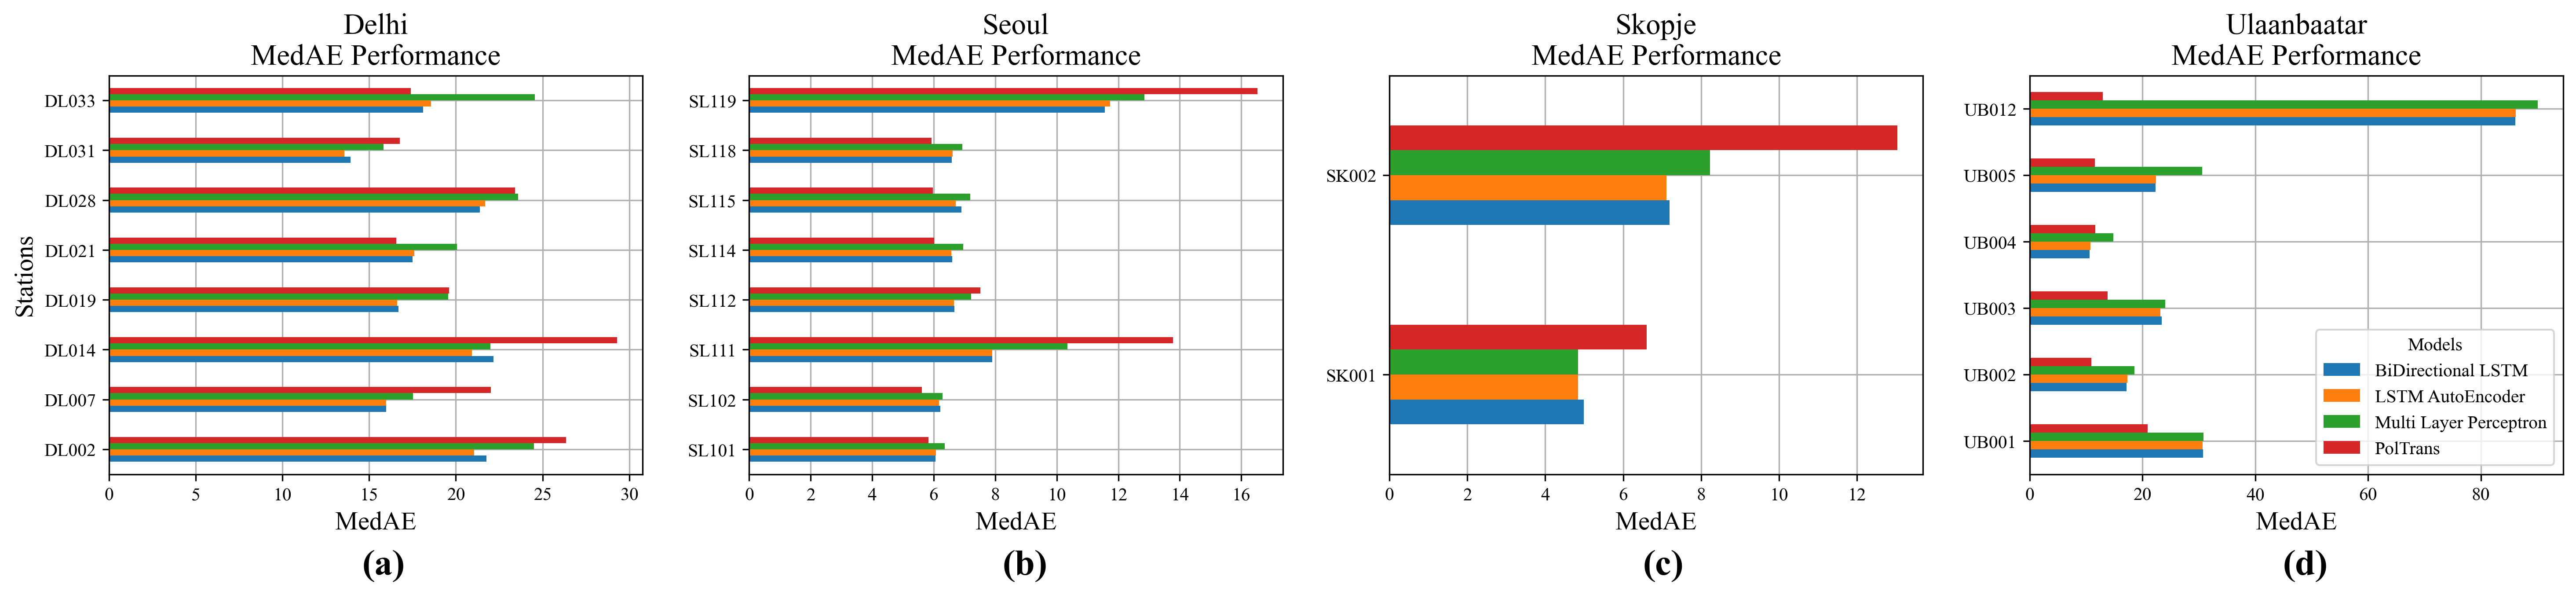
\includegraphics[scale=0.365]{../paper_figures/dl_medae.png}
\caption{MedAE performance of {PolTrans} vs other deep learning models (in $\mu$g/m$^{3}$) for different stations in (a) Delhi, (b) Seoul, (c) Skopje and (d) Ulaanbaatar cities}
\label{fig:dl-medae}
\end{figure*}

\begin{figure*}[h]
\centering
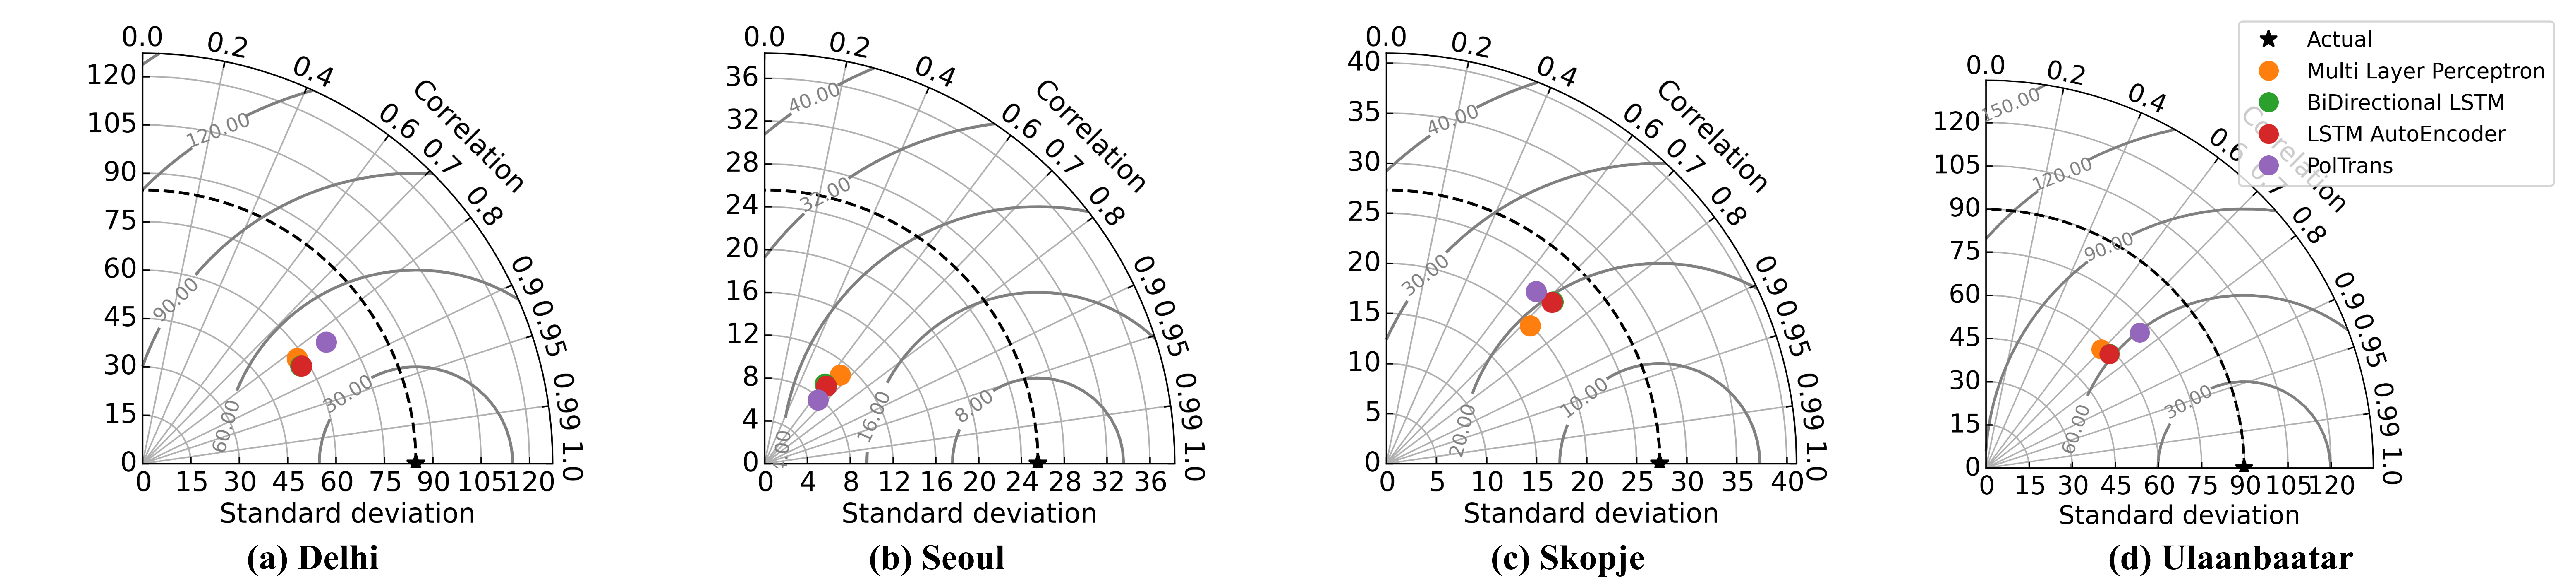
\includegraphics[width=18cm]{../paper_figures/merged_taylor_dl.png}
\caption{Taylor diagrams comparing various deep learning methods vs {PolTrans} for (a) Delhi, (b) Seoul, (c) Skopje and (d) Ulaanbaatar cities}
\label{fig:dl-taylor}
\end{figure*}


\subsubsection{Implementation Details}
For {PolTrans}, because of ReLU, weights were first initialized using Kaiming (He) initialization~\cite{He.2015} method. A ${n_{\text{heads}} = 10}$ for multi-head attention in the encoder layer on extensive experimentation was found to provide optimum results. A learning rate ${\alpha = 5 \times 10^{-3}}$ was used inside an Adam optimizer~\cite{Kingma.2014} with weight decay enabled. A learning rate scheduler with ${\mathrm{stepsize} = 1}$ and ${\gamma = 0.95}$ were taken as parameters to help in faster convergence. For experimental purposes {PolTrans} was trained with ${\mathrm{batchsize} = 64}$ on 200 epochs. The In2Out sequences were constructed with window size ${n = 2}$. For testing purposes, the last 30\% of the original time-samples was used as the test set while the first 70\% was used for training and validation purposes.

\subsubsection{Baselines}
To measure the relative performance increase, three sets of evaluations were carried out. The first of evaluation placed {PolTrans} against popular deep learning methods such as Multi-Layer Perceptron (MLP), Bi-directional LSTM and LSTM Auto-Encoder. The second set and third set of evaluations involved using ML models such as SVM, Polynomial, Linear, Decision Tree and Random Forest regression along with statistical approaches such as ARIMA, AR and Holt-Winters respectively for each type of dataset.
For multivariate datasets, in case of statistical approaches, ARIMAX and ARX were used for their support of exogenous variables. For {PolTrans} the pollutant variable was used to perform modelling and subsequent forecasting in ooth kinds of datasets.

\subsection{Performance in Univariate Time-Series Datasets}

\subsubsection{Comparison with Deep Learning Models}

Upon performing detailed comparisons with various deep learning based methods, {PolTrans} (in terms of RMSE as can be seen in Table \ref{tbl:dl-performance}) was found to outperform comparing deep learning models for Delhi and Ulaanbaatar. The biggest difference in MedAE performance was witnessed in Ulaanbaatar, where {PolTrans} fared significantly better than other deep learning models by a significant margin. For Ulaanbaatar, {PolTrans} managed an RMSE of around 61.167 compared to 64.7-67.6 as in the case for other deep learning methods. In the case of Seoul and Skopje, {PolTrans} performed around 1.09-3.87 units worse in comparison to the best performing deep learning model.

\begin{table}[h]
\small
\centering
\tabcolsep=0.16cm
\caption{Performance metrics averaged over all stations city-wise for deep learning methods and PolTrans}
\label{tbl:dl-performance}
\begin{tabular}{llrrr}
\toprule
City & Model & MAE & RMSE & MedAE \\
\midrule
Delhi & BiDirectional LSTM & 31.958 & 49.658 & 18.439 \\
& LSTM AutoEncoder & \textbf{31.900} & 49.477 & \textbf{18.253} \\
& Multi Layer Perceptron & 34.017 & 51.746 & 20.956 \\
& PolTrans & 33.114 & \textbf{49.020} & 21.426 \\
Seoul & BiDirectional LSTM & 10.891 & 21.716 & 7.312 \\
& LSTM AutoEncoder & \textbf{10.869} & 21.538 & \textbf{7.305} \\
& Multi Layer Perceptron & 11.181 & \textbf{20.936} & 8.017 \\
& PolTrans & 11.855 & 22.597 & 8.398 \\
Skopje & BiDirectional LSTM & \textbf{11.491} & 19.416 & 6.086 \\
& LSTM AutoEncoder & 11.539 & 19.450 & \textbf{5.973} \\
& Multi Layer Perceptron & 11.726 & \textbf{18.942} & 6.533 \\
& PolTrans & 14.435 & 22.126 & 9.820 \\
Ulaanbaatar & BiDirectional LSTM & 43.269 & 64.750 & 31.713 \\
& LSTM AutoEncoder & 43.344 & 64.715 & 31.751 \\
& Multi Layer Perceptron & 46.575 & 67.627 & 34.814 \\
& PolTrans & \textbf{35.200} & \textbf{61.167} & \textbf{13.637} \\
\bottomrule
\end{tabular}
\end{table}

Inspecting the MedAE station-wise performance in Fig.~\ref{fig:dl-medae}, shows that {PolTrans} had mixed results in Delhi and Seoul. In Skopje, {PolTrans} consistently performed worse while in case of Ulaanbaatar, {PolTrans} consistently outperformed all other deep learning models in every station examined. In case of Seoul, for stations, SL119 and SL111, {PolTrans} showed MedAE deviation in the average of around 4 units from the competition. Conversely, in case of Ulaanbaatar, {PolTrans} showed improvements of as much as 60 units for UB012 in comparison. The two versions of LSTM used namely, LSTM Auto-Encoder and Bi-Directional LSTM were found to perform close to each other in almost all stations for all cities with minute differences separating the two.

On examining the Taylor diagrams in Fig.~\ref{fig:dl-taylor}, except in case of Seoul, {PolTrans} showed higher standard deviation in comparison to other deep learning models. Although RMSE and standard deviation performance might have been off w.r.t. competition, the correlation of predicted values in comparison to actual values can be found to be similar without much deviation.

\begin{figure*}[h]
\centering
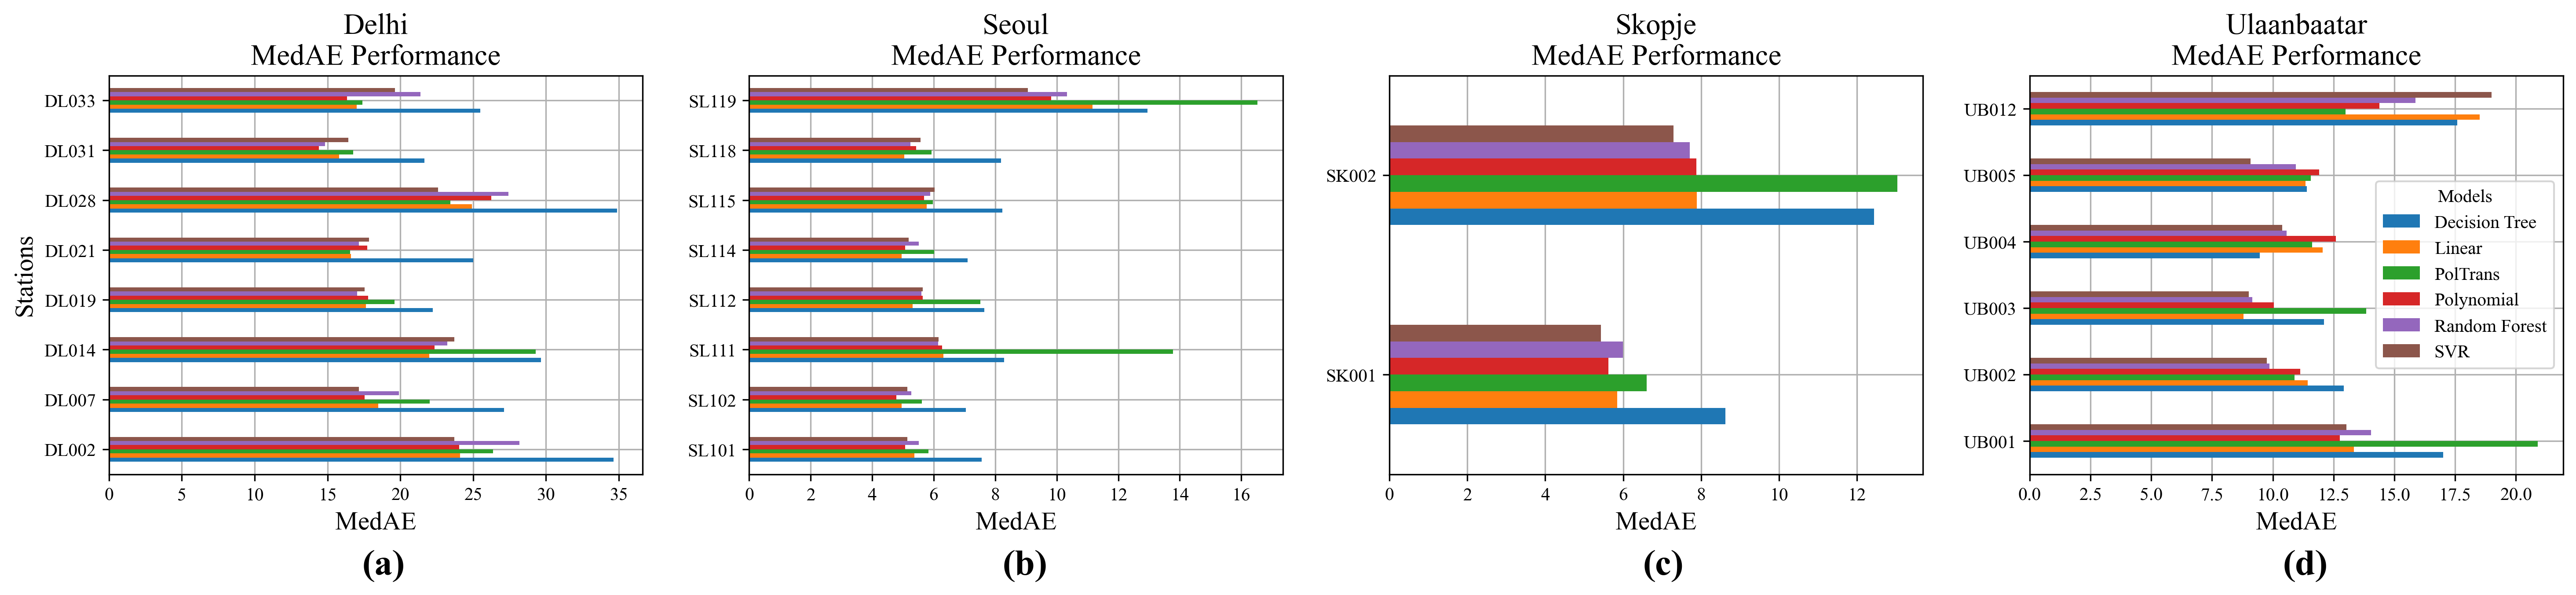
\includegraphics[scale=0.365]{../paper_figures/ml_medae.png}
\caption{MedAE performance of {PolTrans} (indicated in green) vs other machine learning models (in $\mu$g/m$^{3}$) for different stations in (a) Delhi, (b) Seoul, (c) Skopje and (d) Ulaanbaatar cities}
\label{fig:ml-medae}
\end{figure*}

\begin{figure*}[h]
\centering
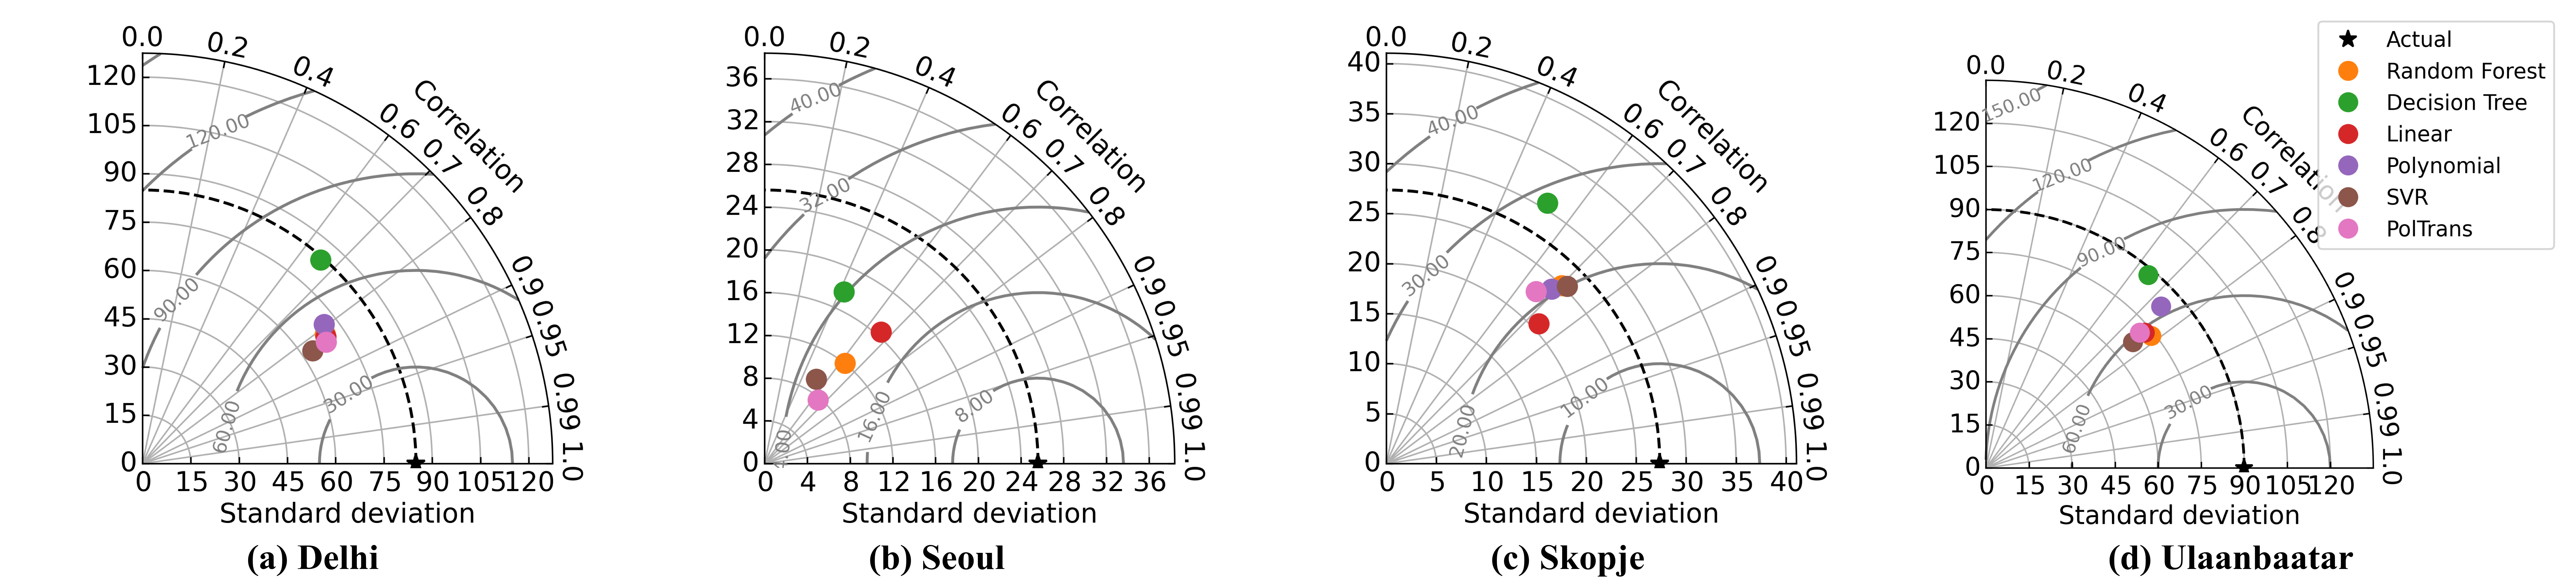
\includegraphics[width=18cm]{../paper_figures/merged_taylor_ml.png}
\caption{Taylor diagrams comparing various machine learning methods vs {PolTrans} for (a) Delhi, (b) Seoul, (c) Skopje and (d) Ulaanbaatar cities}
\label{fig:ml-taylor}
\end{figure*}

\subsubsection{Comparison with Machine Learning Methods}
\label{sec:ml-comp}

In this comparison, as evident from Table \ref{tbl:ml-performance}, {PolTrans} fared worse than its competition in every city examined. Although there does not seem to be present a clear winner, mostly SVR and Random Forest Regression performed the best out of all. Glancing overall comparisons {PolTrans} deviated with RMSE in the 2.19 - 4.09 units range. Out of all models experimented upon, Decision Tree Regression was found to perform the worst with RMSE values off by huge margins when compared to the best performing models.

\begin{table}[h]
\small
\centering
\tabcolsep=0.16cm
\caption{Performance metrics averaged over all stations city-wise for machine learning methods and PolTrans}
\label{tbl:ml-performance}
\begin{tabular}{llrrr}
\toprule
City & Model & MAE & RMSE & MedAE \\
\midrule
Delhi & Decision Tree & 45.666 & 69.912 & 27.575 \\
& Linear & 31.725 & 48.267 & \textbf{19.574 }\\
& PolTrans & 33.114 & 49.020 & 21.426 \\
& Polynomial & 32.703 & 51.767 & 19.556 \\
& Random Forest & 32.667 & 49.121 & 21.138 \\
& SVR & \textbf{31.582} & \textbf{47.862} & 19.828 \\
Seoul & Decision Tree & 13.851 & 25.654 & 8.377 \\
& Linear & 10.269 & \textbf{20.407} & 6.109 \\
& PolTrans & 11.855 & 22.597 & 8.398 \\
& Polynomial & 16.712 & 52.338 & \textbf{5.973} \\
& Random Forest & \textbf{10.253} & 21.175 & 6.186 \\
& SVR & 10.502 & 22.834 & 5.991 \\
Skopje & Decision Tree & 17.365 & 28.644 & 10.532 \\
& Linear & 11.675 & \textbf{18.533} & 6.864 \\
& PolTrans & 14.435 & 22.126 & 9.820 \\
& Polynomial & 12.084 & 20.162 & \textbf{6.751} \\
& Random Forest & 12.185 & 20.502 & 6.852 \\
& SVR & \textbf{11.666} & 19.998 & 6.361 \\
Ulaanbaatar & Decision Tree & 41.375 & 76.775 & 13.412 \\
& Linear & 31.908 & 58.695 & 12.576 \\
& PolTrans & 35.200 & 61.167 & 13.637 \\
& Polynomial & 33.995 & 64.730 & 12.136 \\
& Random Forest & \textbf{31.017} & \textbf{57.071} & \textbf{11.744} \\
& SVR & 31.973 & 60.221 & 11.715 \\
\bottomrule
\end{tabular}
\end{table}

Looking at individual station performances in Fig.~\ref{fig:ml-medae}, although {PolTrans} may not have performed the best, it certainly was also not the worst one being experimented upon. For station UB012, {PolTrans} was the best performing of all machine learning models tested. In majority of the stations, Decision Tree Regression showed the highest MedAE error among all with SVR and Random Forest being the best in almost all stations.

Taylor diagrams for this comparison in Fig. \ref{fig:stat-taylor} show that the performance of machine learning methods (except Decision Tree Regression) and {PolTrans} were close to each other barring a few deviations. One notable observation can be found for Decision Tree Regression, wherein all cities the model consistently showed higher standard deviation coupled with lower correlation scores compared to others.

\subsubsection{Comparison with Statistical Methods}

Analysis of the performance metric in Table \ref{tbl:stat-performance} shows that econometric methods such as AR and ARIMA consistently performed well in all stations experimented on. With RMSE deviations in the range from 1.16 - 4.37 units, {PolTrans} in comparison to statistical methods has been found to lag behind the best performing statistical counterpart by a narrow margin.

\begin{table}[h]
\small
\centering
\tabcolsep=0.16cm
\caption{Performance metrics averaged over all stations city-wise for statistical learning methods and PolTrans}
\label{tbl:stat-performance}
\begin{tabular}{llrrr}
\toprule
City & Model & MAE & RMSE & MedAE \\
\midrule
Delhi & AR & 31.501 & 47.821 & 19.665 \\
& ARIMA & \textbf{30.994} & \textbf{47.234} & \textbf{18.698} \\
& Holt-Winters & 32.021 & 49.848 & 19.041 \\
& PolTrans & 33.114 & 49.020 & 21.426 \\
Seoul & AR & \textbf{10.452} & \textbf{21.431} & \textbf{6.187} \\
& ARIMA & 10.549 & 21.562 & 6.575 \\
& Holt-Winters & 12.102 & 26.199 & 6.711 \\
& PolTrans & 11.855 & 22.597 & 8.398 \\
Skopje & AR & 11.573 & \textbf{18.437} & \textbf{6.490} \\
& ARIMA & \textbf{11.531} & 18.601 & 6.575 \\
& Holt-Winters & 12.560 & 20.496 & 6.614 \\
& PolTrans & 14.435 & 22.126 & 9.820 \\
Ulaanbaatar & AR & 32.491 & 58.698 & 14.128 \\
& ARIMA & \textbf{30.765} & \textbf{56.794} & \textbf{10.911} \\
& Holt-Winters & 31.843 & 59.312 & 11.291 \\
& PolTrans & 35.200 & 61.167 & 13.637 \\
\bottomrule
\end{tabular}
\end{table}

Even though in most stations, {PolTrans} (as evident from Fig. \ref{fig:stat-medae}) has been found to show the highest MedAE error out of all, in specific stations such as DL028 and UB012 in the cities of Delhi and Ulaanbaatar respectively, {PolTrans} has been able to outperform the best performing statistical method used. Although the position of best performing model station-wise was jointly owned by AR, ARIMA and Holt-Winters in proportional amounts, for most of the Ulaanbaatar stations specifically UB012, UB005 and UB004, AR was found to show disproportionally high deviations in MedAE error compared to the competition.

Except Seoul, predictions made by {PolTrans} had correlations close to each other, along 0.6 - 0.8 levels as can be evident from Fig. \ref{fig:stat-taylor}. For Seoul, although correlations between predicted and actual values were almost the same along the 0.6 to 0.7 mark, standard deviations varied a lot, with Holt-Winters and {PolTrans} being on the extreme ends with 24 to 8 units respectively.

\begin{figure*}[h]
\centering
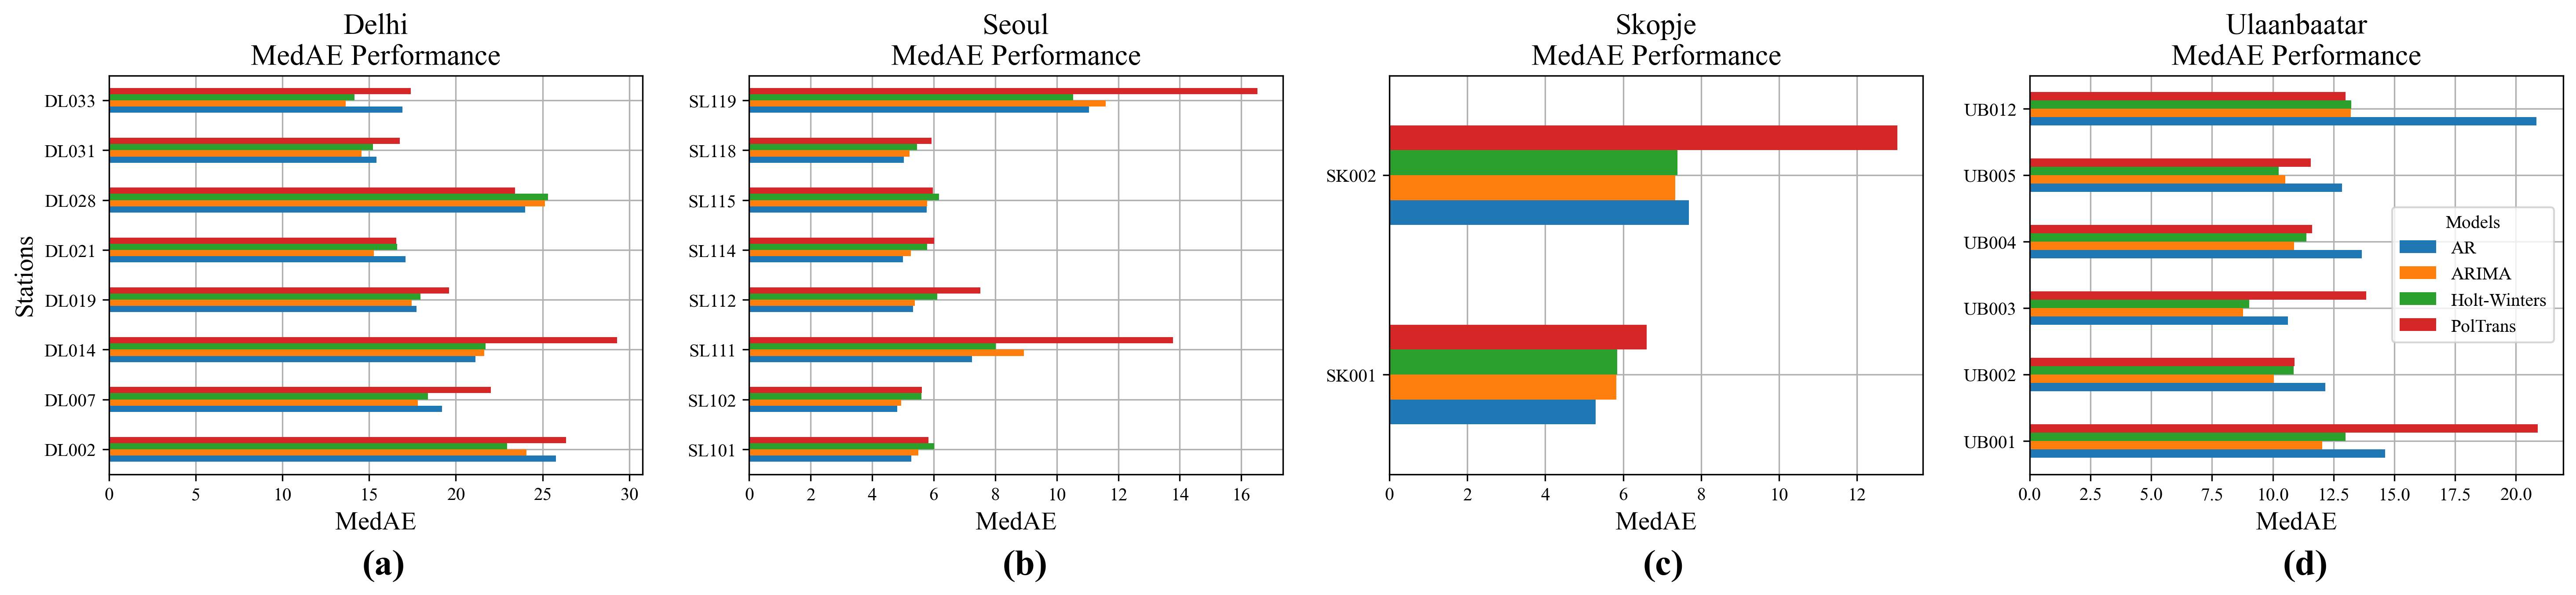
\includegraphics[scale=0.365]{../paper_figures/stat_medae.png}
\caption{MedAE performance of {PolTrans} (indicated in red) vs other statistical models (in $\mu$g/m$^{3}$) for different stations in (a) Delhi, (b) Seoul, (c) Skopje and (d) Ulaanbaatar cities}
\label{fig:stat-medae}
\end{figure*}

\begin{figure*}[h]
\centering
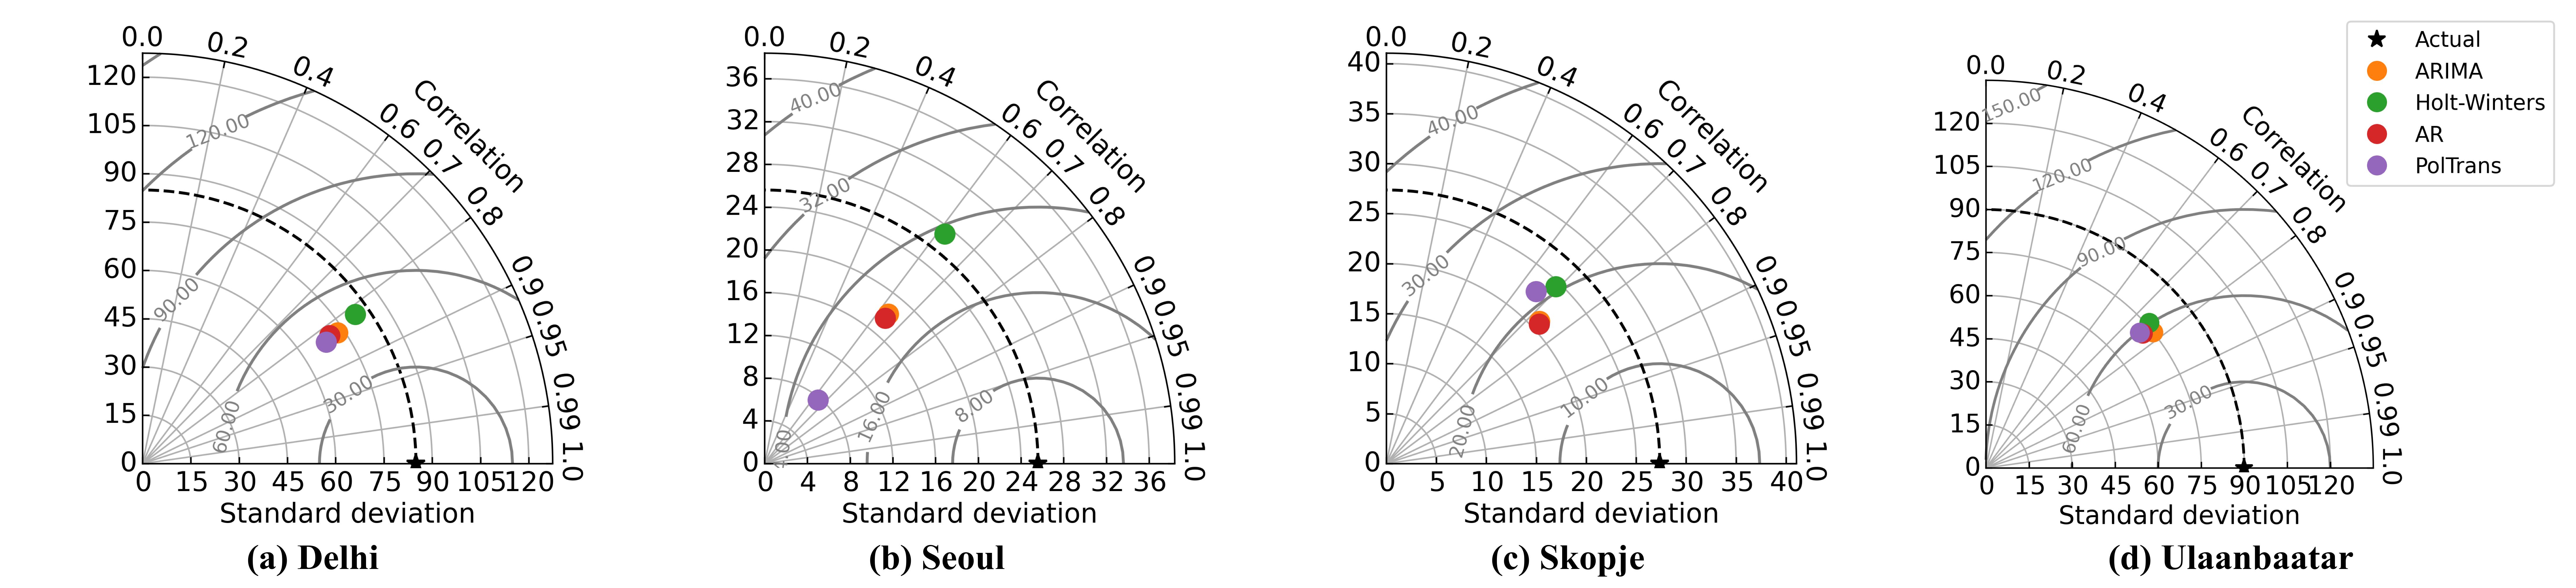
\includegraphics[width=18cm]{../paper_figures/merged_taylor_stat.png}
\caption{Taylor diagrams comparing various statistical methods vs {PolTrans} for (a) Delhi, (b) Seoul, (c) Skopje and (d) Ulaanbaatar cities}
\label{fig:stat-taylor}
\end{figure*}

\subsection{Performance in Mutivariate Time-Series Datasets}

\subsubsection{Comparison with Deep Learning Models}

\begin{table}[h]
\small
\centering
\tabcolsep=0.12cm
\caption{Performance metrics in muti-variate datasets for deep learning methods and PolTrans}
\label{tbl:m_dl-performance}
\begin{tabular}{llrrr}
\toprule
City & Model & MAE & RMSE & MedAE \\
\midrule
Beijing PM${_{10}}$ & BiDirectional LSTM & 56.432 & 83.391 & 39.139 \\
& LSTM AutoEncoder & 50.548 & 70.668 & 40.072 \\
& Multi Layer Perceptron & 50.877 & 70.085 & 42.114 \\
& PolTrans & \textbf{48.725} & \textbf{68.457} & \textbf{35.999} \\
Beijing PM${_{2.5}}$ & BiDirectional LSTM & 54.237 & 75.782 & 39.579 \\
& LSTM AutoEncoder & 51.290 & 71.671 & 38.711 \\
& Multi Layer Perceptron & 48.665 & 64.222 & 41.845 \\
& PolTrans & \textbf{45.161} & \textbf{62.305} & \textbf{34.179} \\
\bottomrule
\end{tabular}
\end{table}

In the case of Beijing PM${_{10}}$ and Beijing PM${_{2.5}}$ multivariate datasets, as evident from Table \ref{tbl:m_dl-performance}, {PolTrans} has been found to outperform other deep learning methods with great margin in all metrics of MAE, RMSE and MedAE. BiDirectional LSTM for both the multivariate Beijing datasets was found to perform consistently worse with RMSE values 83.391 and 75.782 respectively.

\begin{figure}[h]
\centering
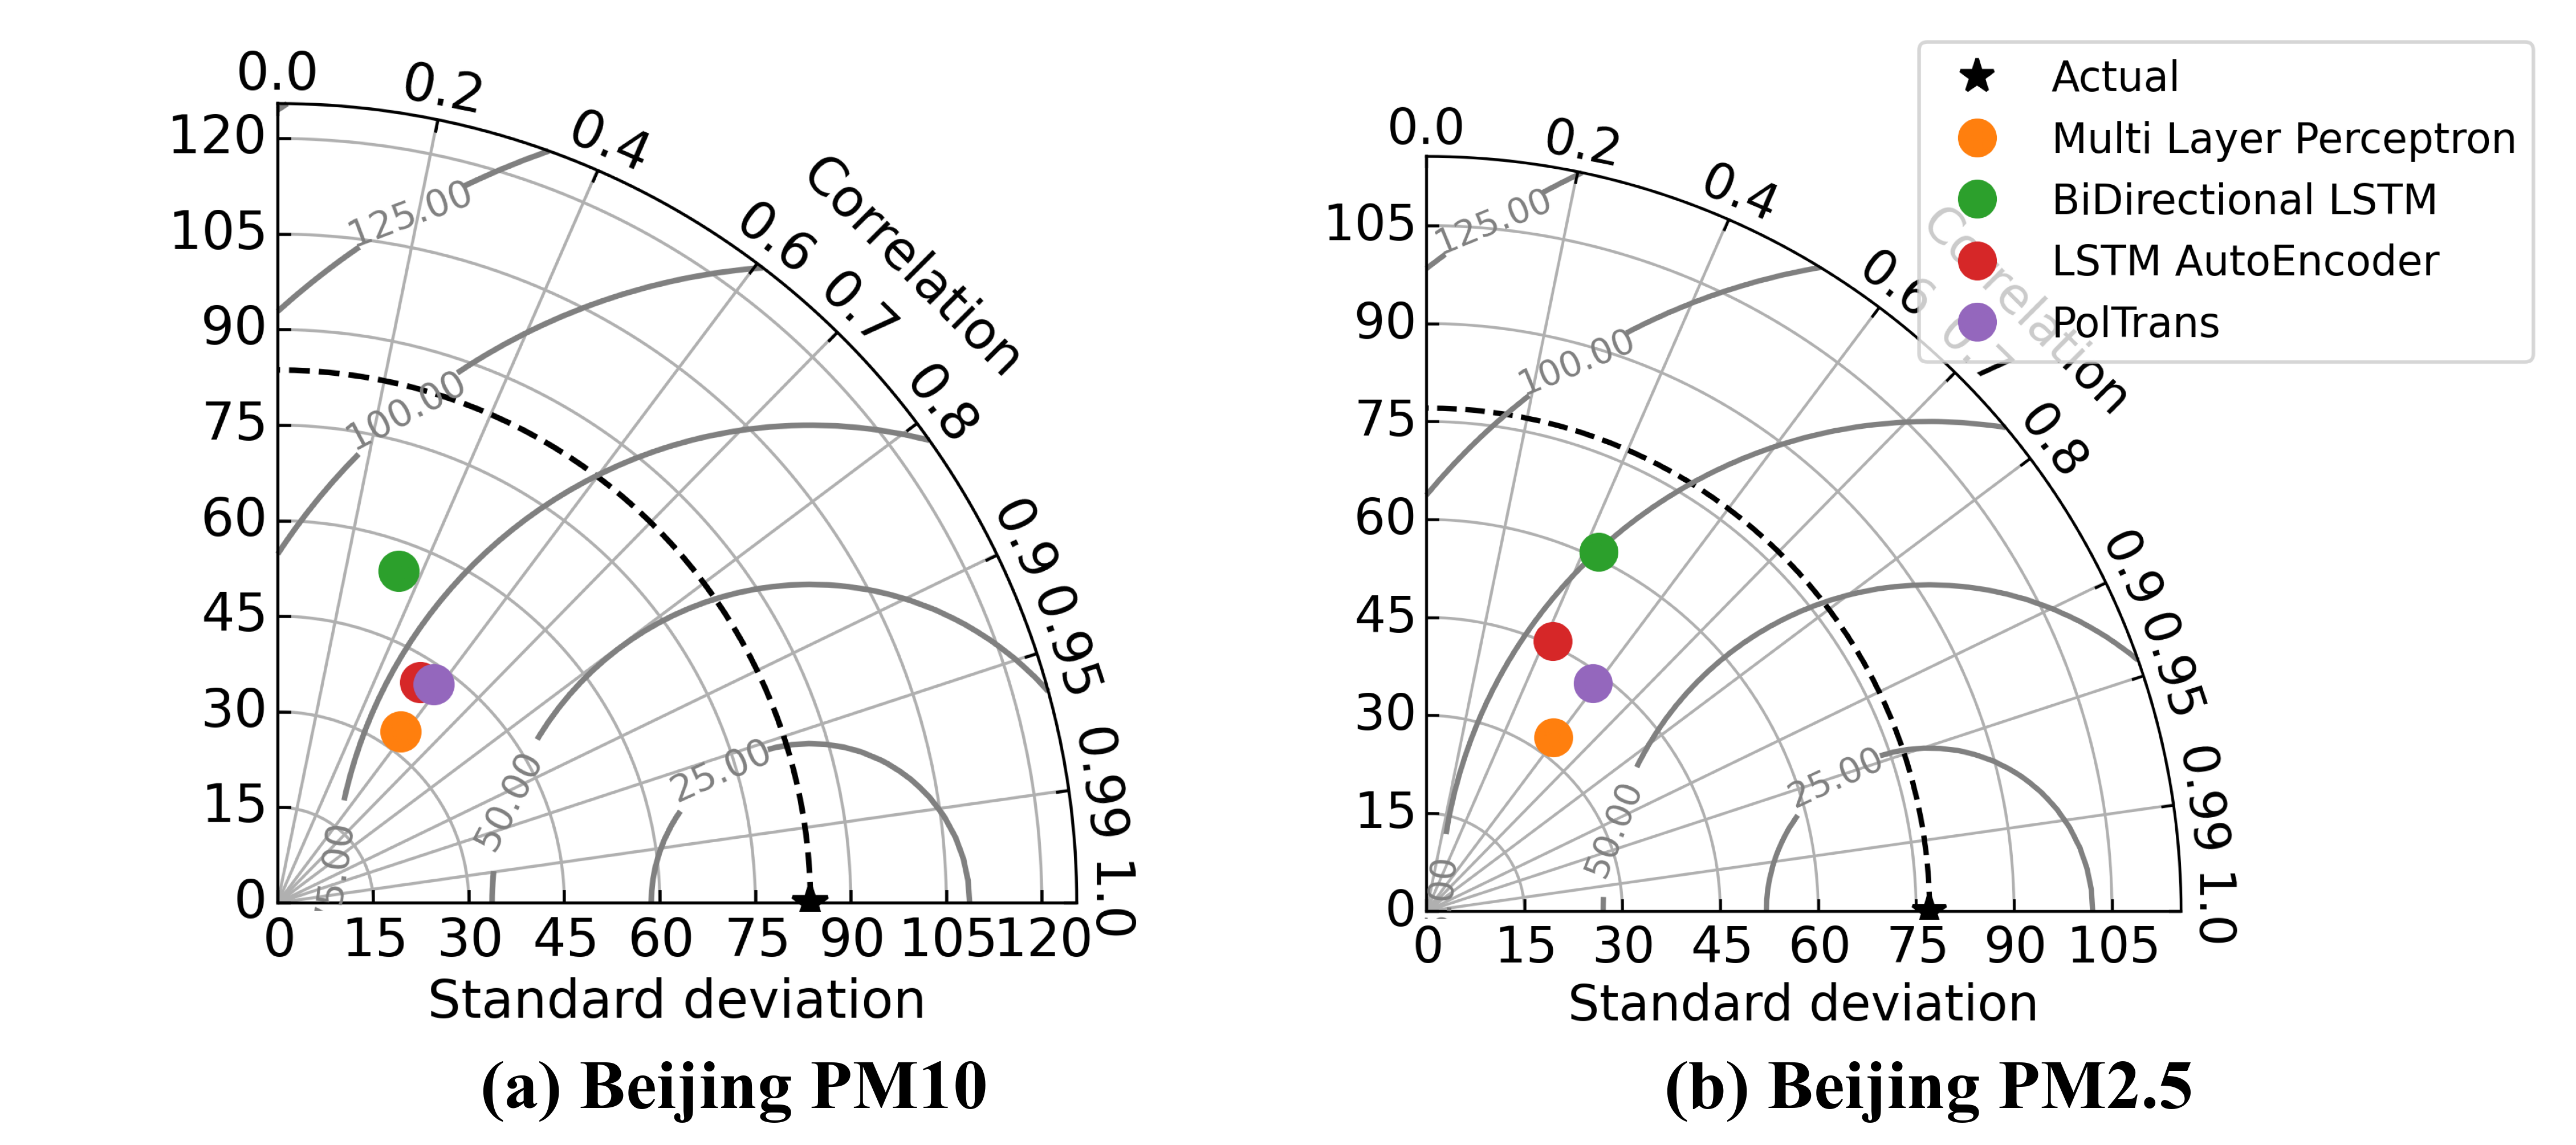
\includegraphics[width=8.5cm]{../paper_figures/merged_taylor_m_dl.png}
\caption{Taylor diagrams comparing various deep learning methods vs {PolTrans} for (a) Beijing PM${_{10}}$ and (b) Beijing PM${_{2.5}}$}
\label{fig:m_dl-taylor}
\end{figure}

For Taylor diagrams in Fig. \ref{fig:m_dl-taylor}, even though most correlation values were in the range 0.6 - 0.7, the correlation for BiDirectional LSTM was found to be a little lower in the middle of 0.3 - 0.4 and alongside exhibited higher standard deviation compared other methods. The Multi Layer Perceptron method was found to show the lowest standard deviation for equivalent correlation values in comparison to the rest.

\subsubsection{Comparison with Machine Learning Models}

Similar to the scenario for univariate datasets mentioned in Section \ref{sec:ml-comp}, {PolTrans} as evident from Table \ref{tbl:m_ml-performance} was unsuccessful in faring better than its machine learning counterparts. With SVR and Polynomial Regression dominating in terms of MAE and RMSE respectively, {PolTrans} was found to be off by around 2.7 units in RMSE and 0.75 units in MAE compared to the best performing counterparts. Out of all, Decision Tree Regression was found to perform worse in terms of RMSE and MAE with huge margins in comparison to others.

\begin{table}[h]
\small
\centering
\tabcolsep=0.16cm
\caption{Performance metrics in muti-variate datasets for machine learning methods and PolTrans}
\label{tbl:m_ml-performance}
\begin{tabular}{llrrr}
\toprule
City & Model & MAE & RMSE & MedAE \\
\midrule
Beijing PM${_{10}}$ & Decision Tree & 61.370 & 87.291 & 43.240 \\
& Linear & 48.372 & 67.374 & 36.312 \\
& PolTrans & 48.725 & 68.457 & 35.999 \\
& Polynomial & 47.474 & \textbf{66.626} & 36.055 \\
& Random Forest & 49.589 & 70.555 & 37.424 \\
& SVR & \textbf{47.130} & 69.578 & \textbf{32.953} \\
Beijing PM${_{2.5}}$ & Decision Tree & 56.388 & 81.938 & 37.395 \\
& Linear & 44.928 & 61.244 & 34.881 \\
& PolTrans & 45.161 & 62.305 & 34.179 \\
& Polynomial & 43.586 & \textbf{59.532} & 34.757 \\
& Random Forest & 44.485 & 61.574 & 32.474 \\
& SVR & \textbf{42.830} & 61.028 & \textbf{30.583} \\
\bottomrule
\end{tabular}
\end{table}

A similar picture prevailed for Taylor diagrams as well in Fig. \ref{fig:m_ml-taylor}. With Decision Tree Regression being left with a lower correlation in the 0.4 - 0.6 level and higher standard deviation around the 75 mark, other models clustered at standard deviation levels of 45 units with correlations in the 0.6 - 0.7 levels.

\begin{figure}[h]
\centering
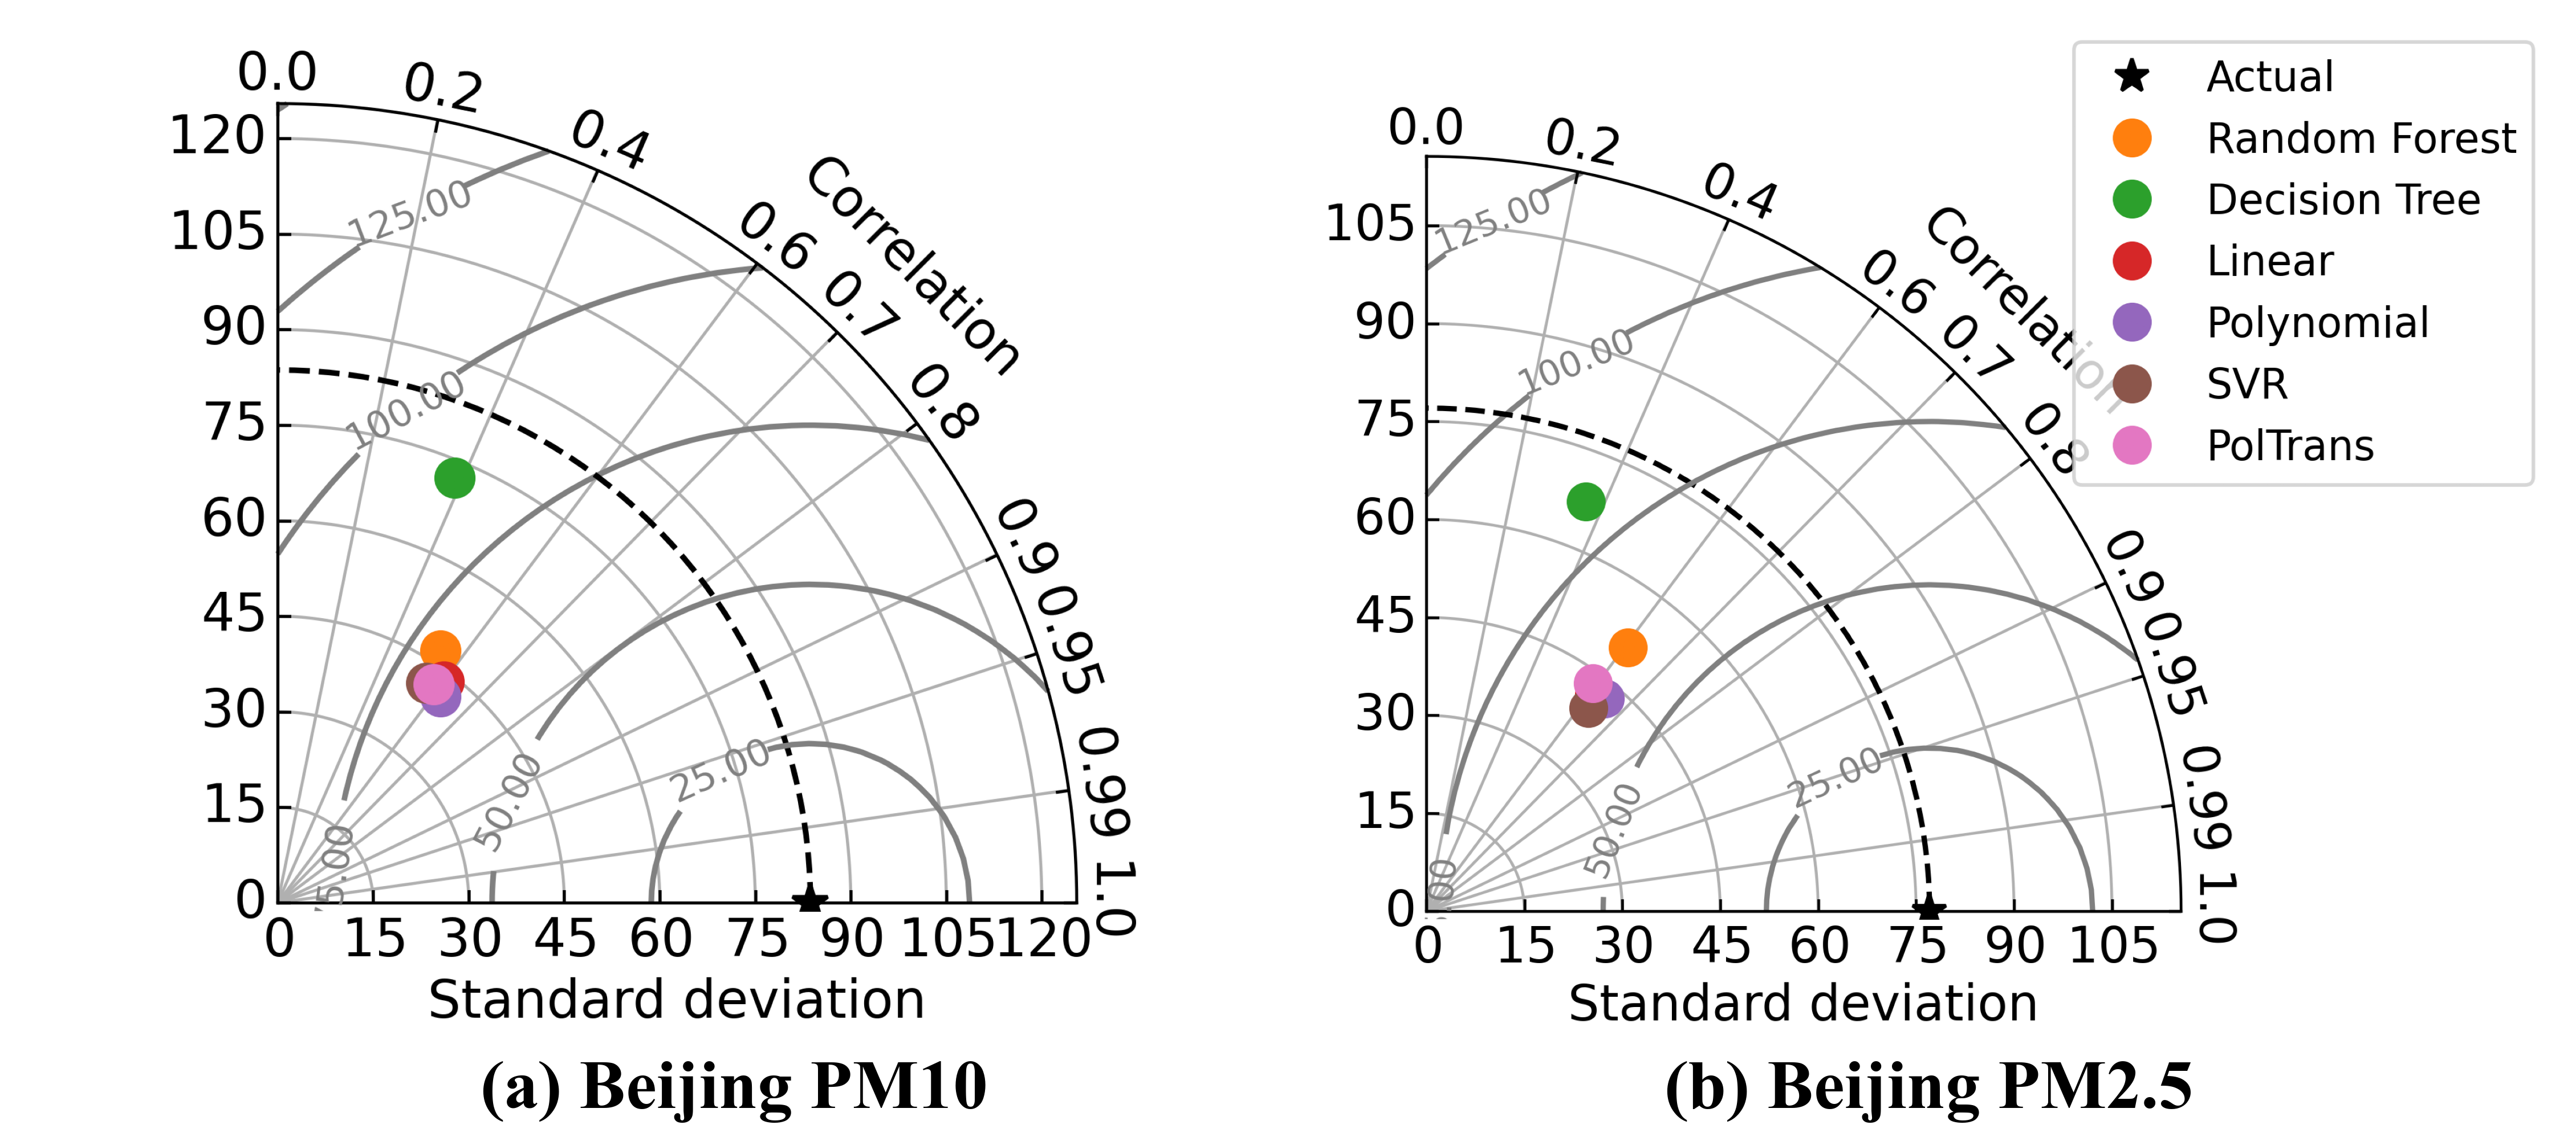
\includegraphics[width=8.5cm]{../paper_figures/merged_taylor_m_ml.png}
\caption{Taylor diagrams comparing various machine learning methods vs {PolTrans} for (a) Beijing PM${_{10}}$ and (b) Beijing PM${_{2.5}}$}
\label{fig:m_ml-taylor}
\end{figure}

\subsubsection{Comparison with Statistical Learning Models}

The exogenous equipped ARIMAX outperformed all other models used in this specific comparison, as can be seen in Table \ref{tbl:m_stat-performance}. {PolTrans} was the worst performer of all three with a margin of 12 - 13 units in MAE and 14 - 15 units in RMSE errors. Although ARX was not the worst performing model in the experiments, the difference in the performance metrics for ARX was lower compared to PolTrans and was close in the 5 - 6 units interval for MAE and RMSE.

\begin{table}[h]
\small
\centering
\tabcolsep=0.16cm
\caption{Performance metrics in muti-variate datasets for statistical learning methods and PolTrans}
\label{tbl:m_stat-performance}
\begin{tabular}{llrrr}
\toprule
City & Model & MAE & RMSE & MedAE \\
\midrule
Beijing PM${_{10}}$ & ARIMAX & \textbf{36.718} & \textbf{54.600} & \textbf{25.198} \\
& ARX & 41.590 & 60.391 & 29.748 \\
& PolTrans & 48.725 & 68.457 & 35.999 \\
Beijing PM${_{2.5}}$ & ARIMAX & \textbf{32.750} & \textbf{47.804} & \textbf{22.407} \\
& ARX & 37.428 & 52.983 & 27.033 \\
& PolTrans & 45.161 & 62.305 & 34.179 \\
\bottomrule
\end{tabular}
\end{table}

The Taylor diagrams in Fig. \ref{fig:m_stat-taylor} show a noticable difference in the model performance for ARIMA, ARX and {PolTrans}. While {PolTrans} had correlation values around the 0.6 range, ARX and ARIMAX had values in the 0.7 and 0.8 mark. Regarding standard deviation, {PolTrans} showed lower values within 30 - 45 while ARX and ARIMAX had values ranging in 45 - 60 and 60 - 75 respectively.

\begin{figure}[h]
\centering
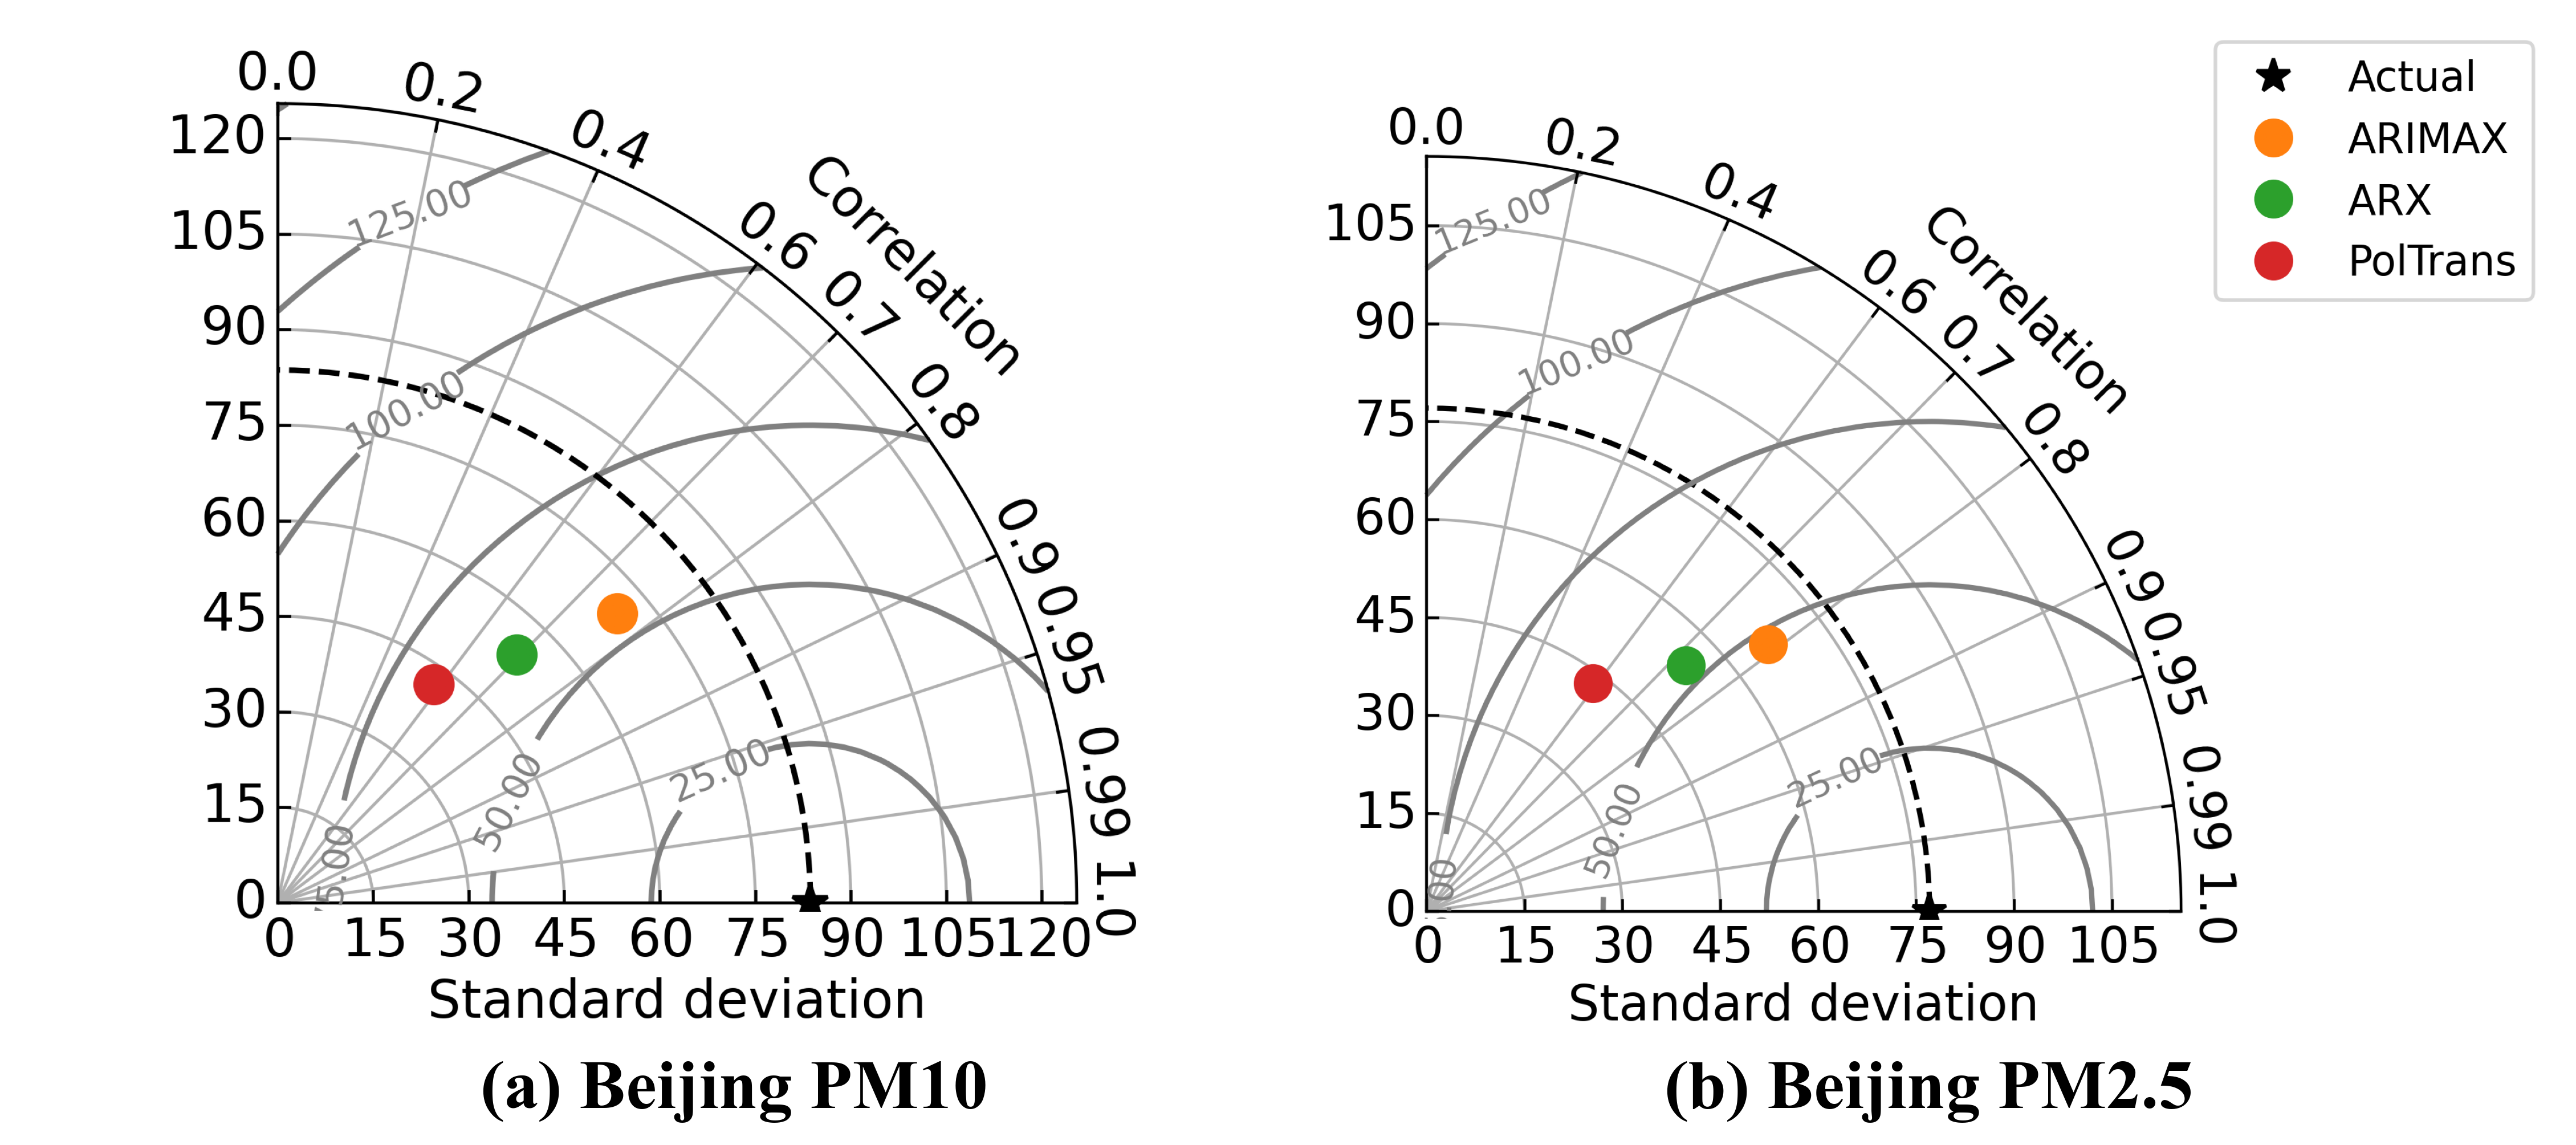
\includegraphics[width=8.5cm]{../paper_figures/merged_taylor_m_stat.png}
\caption{Taylor diagrams comparing various statistical methods vs {PolTrans} for (a) Beijing PM${_{10}}$ and (b) Beijing PM${_{2.5}}$}
\label{fig:m_stat-taylor}
\end{figure}

\subsection{Discussion}

\begin{figure*}[h]
\centering
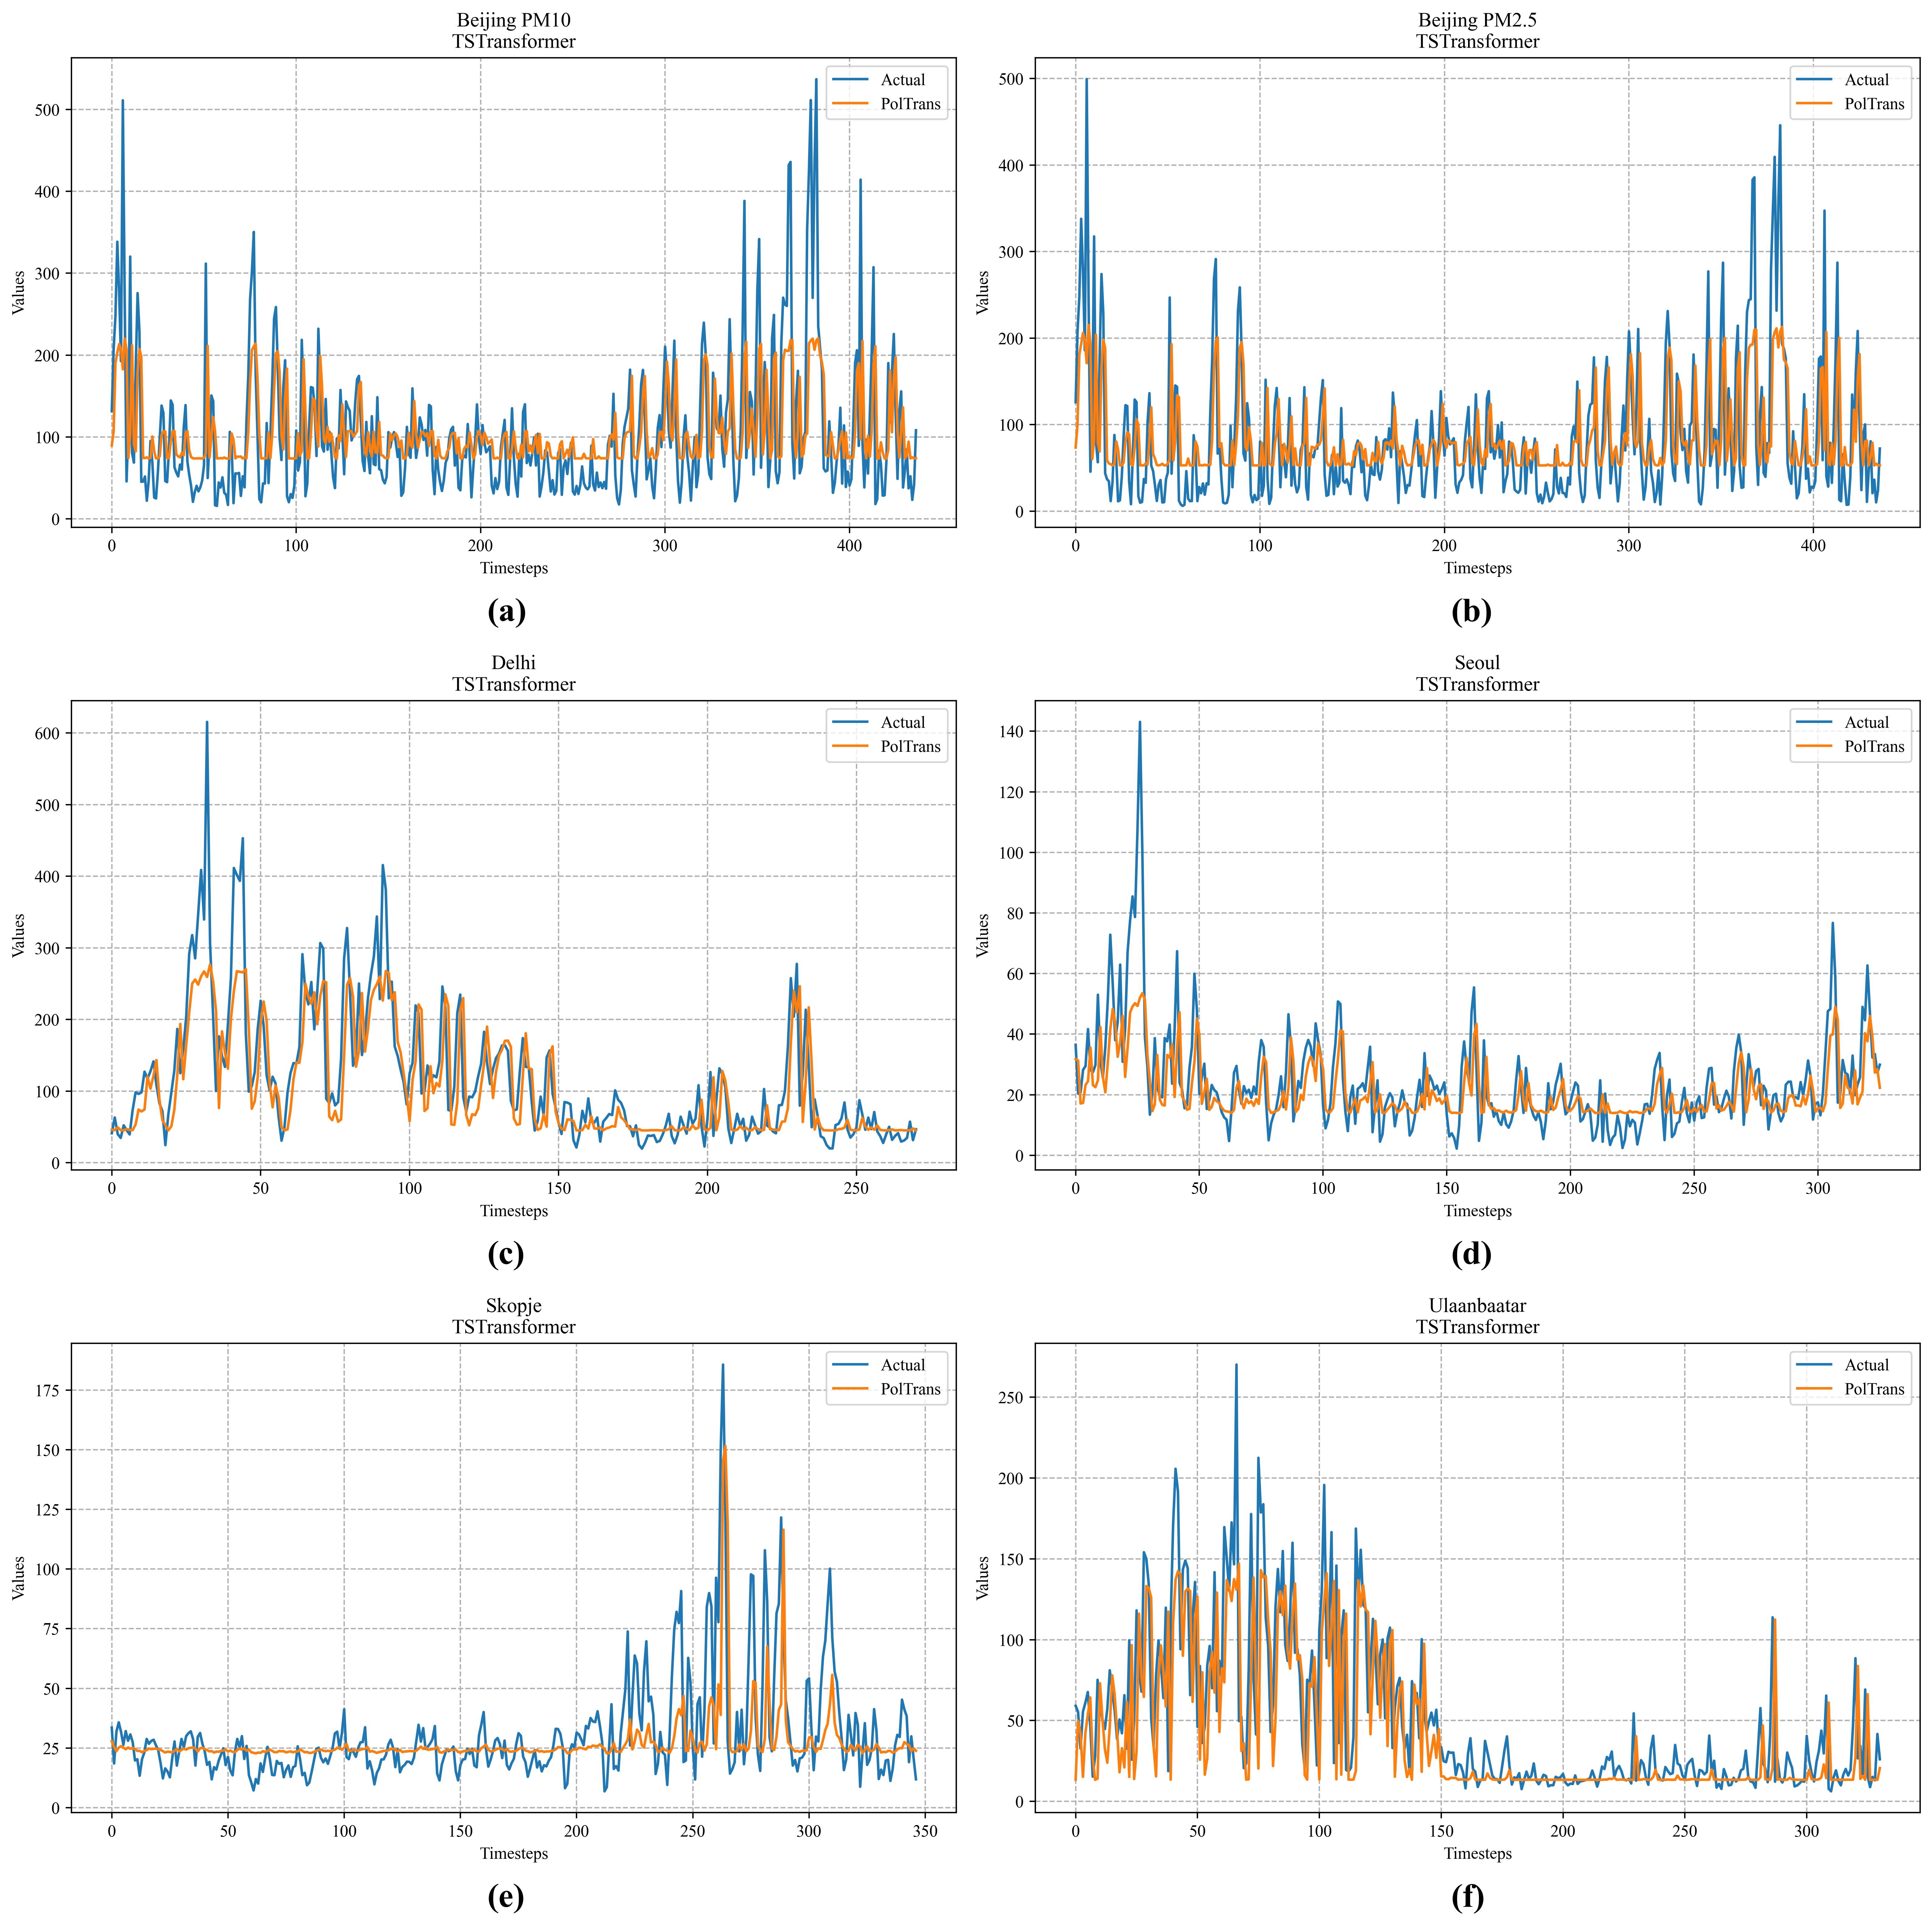
\includegraphics[width=16cm]{../paper_figures/ts-lineplot.png}
\caption{Line plots demonstrating predictions made by {PolTrans} (indicated in orange) vs actual PM${_{2.5}}$ / PM${_{10}}$ count as reported (in $\mu$g/m$^{3}$) for (a) Beijing PM${_{10}}$, (b) Beijing PM${_{2.5}}$ and a sample station in each of (c) Delhi, (d) Seoul, (e) Skopje and (f) Ulaanbaatar datasets}
\label{fig:ts-linepots}
\end{figure*}

From the extensive experimentation performed in testing {PolTrans} against multiple baselines from areas of deep learning, machine learning and statistical methods, although {PolTrans} shows great promise as a deep learning method in forecasting time-series data in the pollution domain, other methods in the statistical and machine learning group of models perform better in the performance metrics used. However, the biggest advantage {PolTrans} benefits from lies in its ability to rapidly train (w.r.t. other deep learning methods) as well as parallelize in distributed settings. When the volume of data increases (order ${>= 10{^{6}}}$), statistical methods such as ARIMA, Holt-Winters, etc. take higher training times due to their inherent modelling characteristics.

Looking at the nature of predictions produced by {PolTrans} in Fig. \ref{fig:ts-linepots}, where ordinary deep learning models normally succumb to high variability and often lead to projections close to the mean, {PolTrans} was successfully able to model the variability fairly and predict with greater accuracy.

Although the pollutants in focus were PM${_{2.5}}$ and PM${_{10}}$, similar results could be expected in case of other major pollutants for different cities. In the experiments, the chief focus was made to pick cities which had high variation in pollution counts. In urban environments where the pollution scenario is relatively stable and shows regular periodicity (eg. New York City, London, Washington DC, etc.), {PolTrans} as well as other methods experimented, would help in production of much more refined and accurate insights with relatively higher accuracy.

\section{Conclusion}
\label{sec:conclusion}

In this paper, a transformer based deep learning approach (termed in this paper as {PolTrans}) based on the popular NLP Transformer was experimentally evaluated with respect to multiple baseline methods from statistical, machine learning and deep learning domains which are widely used in pollution modelling. The experiments ran on both univariate and multivariate datasets belonging to different major cities all around the world. The results show that although {PolTrans} show good progress in comparison to other commonly used deep learning approaches such as BiDirectional LSTM, LSTM Auto-Encoder, MLP, etc. it still lags in comparison to machine learning and statistical approaches such as SVR, ARIMA, Holt-Winters, etc.

It is hoped that such a comparative evaluation made in this paper with different key urban settings in focus, will assist concerned policymakers (especially those working under SDG 11 and 13) in selecting appropriate pollution modelling strategies to gauge their own pollution scenarios effectively.

\section*{Data and Code Availability}
The analysis code and data used for this paper can be found in the following link - \url{https://github.com/nathzi1505/PolTrans-Comparative-Study}. [Note: Since the repository is currently private due to confidential reasons, please email requesting for permission].

\section*{Acknowledgment}
I am extremely thankful to Asif Iqbal Middya (Asif da) for taking out time to resolve doubts that came up as the project progressed. Needless to say the project would not be possible without his extensive mentorship and guidance. 

\ifCLASSOPTIONcaptionsoff
\newpage
\fi

\bibliographystyle{IEEEtran}
\bibliography{bibliography}

\end{document}